% !TEX root = paper.tex
% !TeX spellcheck = en_US

\section{Modeling Matrix Multiplication}
\label{sec:ModelMatMult}
In this section, we detail the optimization of matrix multiplication on modern CPUs. We start with the implementation of dense-dense matrix multiplication (DMM) and then we move to the sparse-dense (SDMM) matrix case. Matrix multiplication has a prominent role in a wide spectrum of scientific applications (linear algebra, physics, economics, engineering), and it also represents the structural operation in neural network forward and backward pass. We believe that, when dealing with the efficiency-effectiveness trade-off, a comprehensive analysis of the underlying multiplication mechanisms is essential. We develop time predictors for matrix multiplication both in the dense and in the sparse domain, and we then jointly apply them to develop an analytical model that estimates the scoring time of a neural network given the matrix shapes and the sparsity percentage of each layer of the Feed Forward Network (FFN). Our predictors are analytic, \textit{i.e.}, not learned, and they are based on 1) the knowledge gained from the implementation of DMM and SDMM on modern CPU architectures, 2) empirical measurements showing the performance of CPU on these operations under different conditions. 
 We observe that, by exploiting the predictors we are proposing, we are allowed to train only the architectures that match the desired efficiency constraints. In a latency-bound application, the efficiency constraints are specified in the requirements. In an effectiveness-oriented context, they can be inferred by observing the execution time of the competitor, \textit{i.e.}, ensembles of tree-based models. As a consequence, the use of our predictors allows to significantly reduce the search space of the optimal architecture. Furthermore, our predictors are task-agnostic, hence they can be applied in any Feed Forward Network (FFN) application field.

%It is worth noting that the time predictors that we develop can have implications that go beyond this ranking-oriented use case and possibly generalize to all the FFN application fields.
%\fnote{non ho capito ultima frase. spiega meglio. FM}
%Todo quello che consente di fare il modello matematico per la predizione dei tempi potrebbe essere una lista dentro un enumerate.. per adesso me ne  é venuto in mente uno solo

\subsection{Dense Matrix Multiplication}
\label{subsec:dmm}
In this section, we investigate how Dense Matrix Multiplication (DMM) is optimized on modern CPUs. DMM has countless applications, hence lots of effort has been spent to attain fast implementations. The current state-of-the-art algorithm for DMM is the the well-known Goto Algorithm~\cite{goto2008anatomy}, on which are based several open (GotoBLAS~\cite{goto2008anatomy}, OpenBLAS~\cite{xianyi2012openblas}, BLIS~\cite{huang2016blislab}) or commercial (Intel MKL~\cite{wang2014intel}) implementations.
%During the last 30 years, a major effort has been made in developing CPU-oriented optimizations, exploiting cache hierarchy, vector instructions and pre-fetching. The main precepts are contained into the third level of the Basic Linear Algebra Subprograms (BLAS) library; these precepts are based on the well-known Goto Algorithm~\cite{goto2008anatomy}, which is also the established state of the art for dense matrix multiplication. In fact,  
%The world famous Basic Linear Algebra Subprograms (BLAS)~\cite{lawson1979basic}, for example, has its own 3-level routines entirely dedicated to matrix-matrix operations. 
%several open (GotoBLAS~\cite{goto2008anatomy}, OpenBLAS~\cite{xianyi2012openblas}, BLIS~\cite{huang2016blislab}) or commercial (Intel MKL~\cite{wang2014intel}) implementations are now available, all developed according to the Goto algorithm for blocked matrix multiplication~\cite{goto2008anatomy}.

The multiplication of two $ n \times n$ dense matrices involves $\mathcal{O}(n^3)$ floating-point operations with $\mathcal{O}(n^2)$ data, as can be easily evicted from Equation~\ref{eq:mmdef}. In modern processors, the interaction with memory is more time-consuming than the  computation itself (\textit{memory bandwidth bottleneck}), but a wise memory management allows to amortize the data movement over a large number of computations.
The mathematical definition of matrix multiplication is the following: given  $A \in \mathbb{R}^{m \times k}$, $B \in \mathbb{R}^{k \times n}$, the matrix multiplication binary operator computes $C = A*B$  with $C \in \mathbb{R}^{m \times n}$, where every element of $C$ is given by

\begin{equation} \label{eq:mmdef} 
C_{i,j} = \sum_{p=1}^{k} A_{i, p}  B_{p,j} \qquad  i=1, \dots, m \quad j=1, \dots, n 
\end{equation}
The Goto Algorithm consists of iteratively decomposing the overall DMM into a series of smaller matrix operations in a cache-aware fashion, until matrices fit the CPU registers. Then matrices are multiplied by means of a highly engineered \textit{micro-kernel}. We now provide a breakdown of the Goto Algorithm as implemented in the BLIS library~\cite{lawson1979basic,van2015blis}, which assumes the CPU to be equipped with 3 levels of cache and vectorized instructions. The first three steps of the blocked matrix multiplication algorithm are depicted in Figure~\ref{fig:gotofirst}.

\begin{figure}[htb]
	\centering
	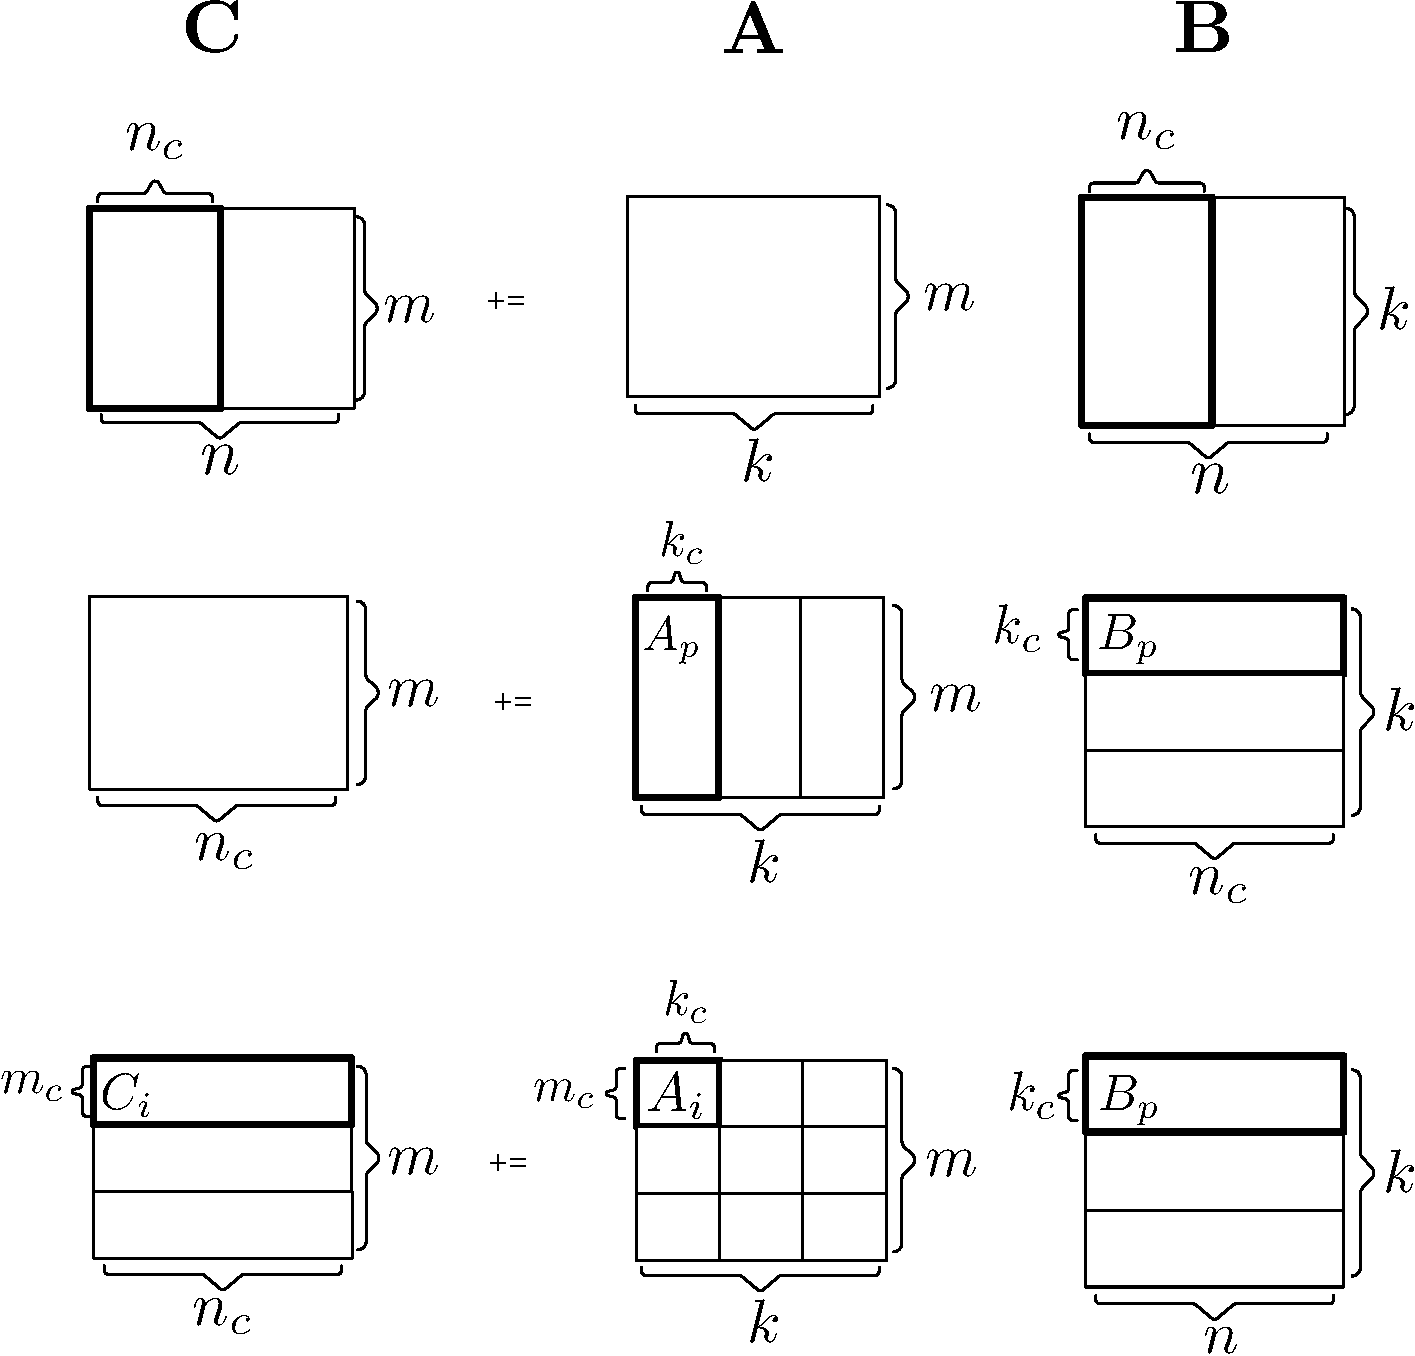
\includegraphics[width=\columnwidth]{imgs/Goto_first.pdf}
	\caption{First three steps of the Goto algorithm for Dense Matrix multiplication.}
		\label{fig:gotofirst}
\end{figure}

The blocked matrix multiplication algorithm begins by partitioning along the columns of $C$ and $B$ into blocks of size $n_c$, obtaining  sub-matrices of $C$ of shape $m \times n_c$ and sub-matrices of $B$ of shape $k \times n_c$. Each $C$ sub-matrix is obtained by multiplying the complete $A$ matrix with the corresponding sub-matrix of $B$. Then, the procedure partitions the columns of $A$ and the rows of $B$ into blocks of size $k_c$, to obtain $A_p$, \textit{i.e.}, vertical panels of size $m \times k_c$, and $B_i$, \textit{i.e.}, horizontal panels of size $k_c \times n$. The $B_i$ panels are packed into the L3 cache reordering data according to a specific pattern which allows to access data contiguously even after the subsequent partitions.  We adopt the notation $\tilde{X}$ to indicate that the sub-matrix $X$ respects this pattern. Observe that, after the blocking on the $k$ axis, the original multiplication is boiled down into a series of rank-k updates so that $C = C + A_p B_p$. A further partition is performed along rows of $A$, with size $m_c$, generating $C_i$ and $A_i$. $A_i$ is, as was $B_i$ previously, packed into $\tilde{A_i}$ in the L2 cache.

% \begin{figure}[htb]
% 	\centering
% 	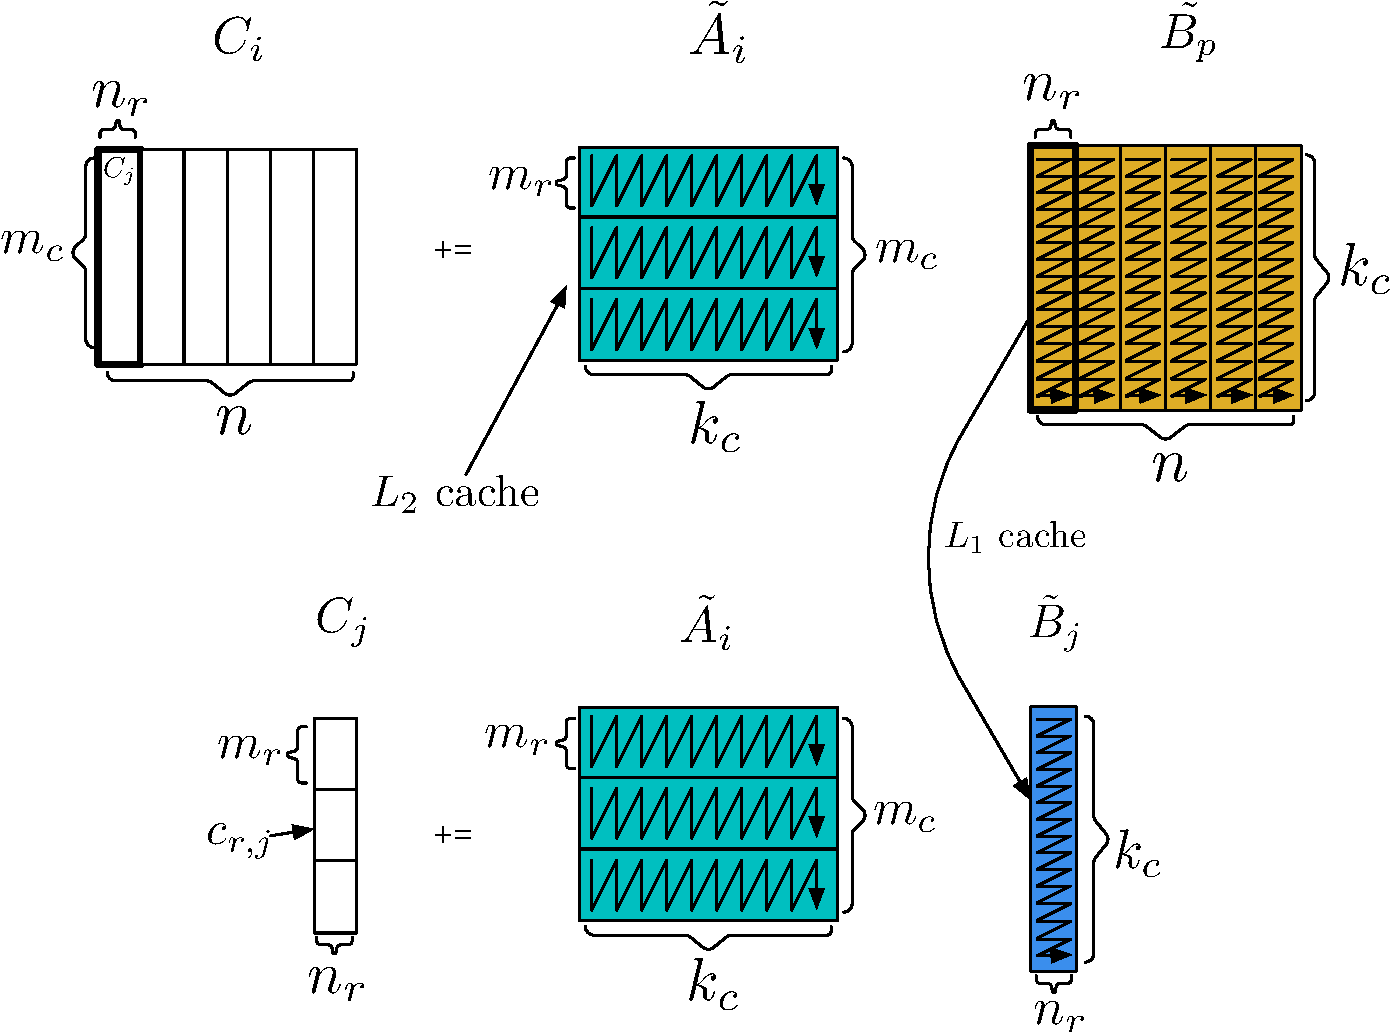
\includegraphics[width=\columnwidth ]{imgs/Goto_second.pdf}
% 		\caption{Macro-Kernel in the Goto algorithm for Dense Matrix Multiplication (DMM).}
% 		\label{fig:gotosecond}
% \end{figure}

%\fnote{sistema caption della figura sopra. metti sempre i punti alla fine delle caption. controlla ovunque. FM}

\noindent \textbf{Macro-Kernel}. The macro-kernel, or inner kernel as in the original algorithm by Goto \textit{et al.}~\cite{goto2008anatomy}, is responsible for orchestrating the memory movement between the RAM memory and the caches. Let us consider the operation $C_i \leftarrow C_i +  \tilde{A}_i*  \tilde{B}_p $, with $C_i$ of size $m_c \times n$, $\tilde{A}_i$ of size $m_c \times k_c$ and $\tilde{B}_p$ of size $k_c \times n$. The macro kernel decomposes this operation into a series of block-panel multiplications, as shown in Figure~\ref{fig:gotosecond}. As aforementioned, both $\tilde{A}_i$ and $ \tilde{B}_p$ are packed with a special pattern, indicated by the arrows in Figure~\ref{fig:gotosecond}. In particular, $\tilde{A}_i$ is organized into sub-matrices $\tilde{A}_j$ of size $m_r \times k_c$, with elements stored in column-major order, while $ \tilde{B}_p$ is organized in panels of size $k_c \times n_r$, stored in row-major order, named $\tilde{B}_j$. This data access pattern reflects the order in which the micro-kernel accesses data. 

Goto \textit{et al.}~\cite{goto2008anatomy} observed the advantages of packing $\tilde{A}_i$ into the L2 cache. The ratio between FLOPs and memory operations, regardless if the original data rely in L3 cache or in main memory, can be modeled as
 $$ \frac{2 m_{c} k_{c}}{\left(2 m_{c}+k_{c}\right)} $$
if $k_c << n$.
Hence, the higher is the $m_c k_c$ product, the smaller is the overhead of memory transfer on the overall computation. 
Knowing that L2 cache is larger than L1, we can afford larger $m_c$ and $k_c$ values \footnote{In the original work, Goto et al.~\cite{goto2008anatomy} point out that $C_i \leftarrow C_i +  \tilde{A}_i  \tilde{B}_p $ should be computed at the peak rate of CPU. This condition is true if all three matrices reside in L1 cache, but it can be considered true even if $\tilde{A}_i$ is in L2.}.


\begin{figure}
	\centering
	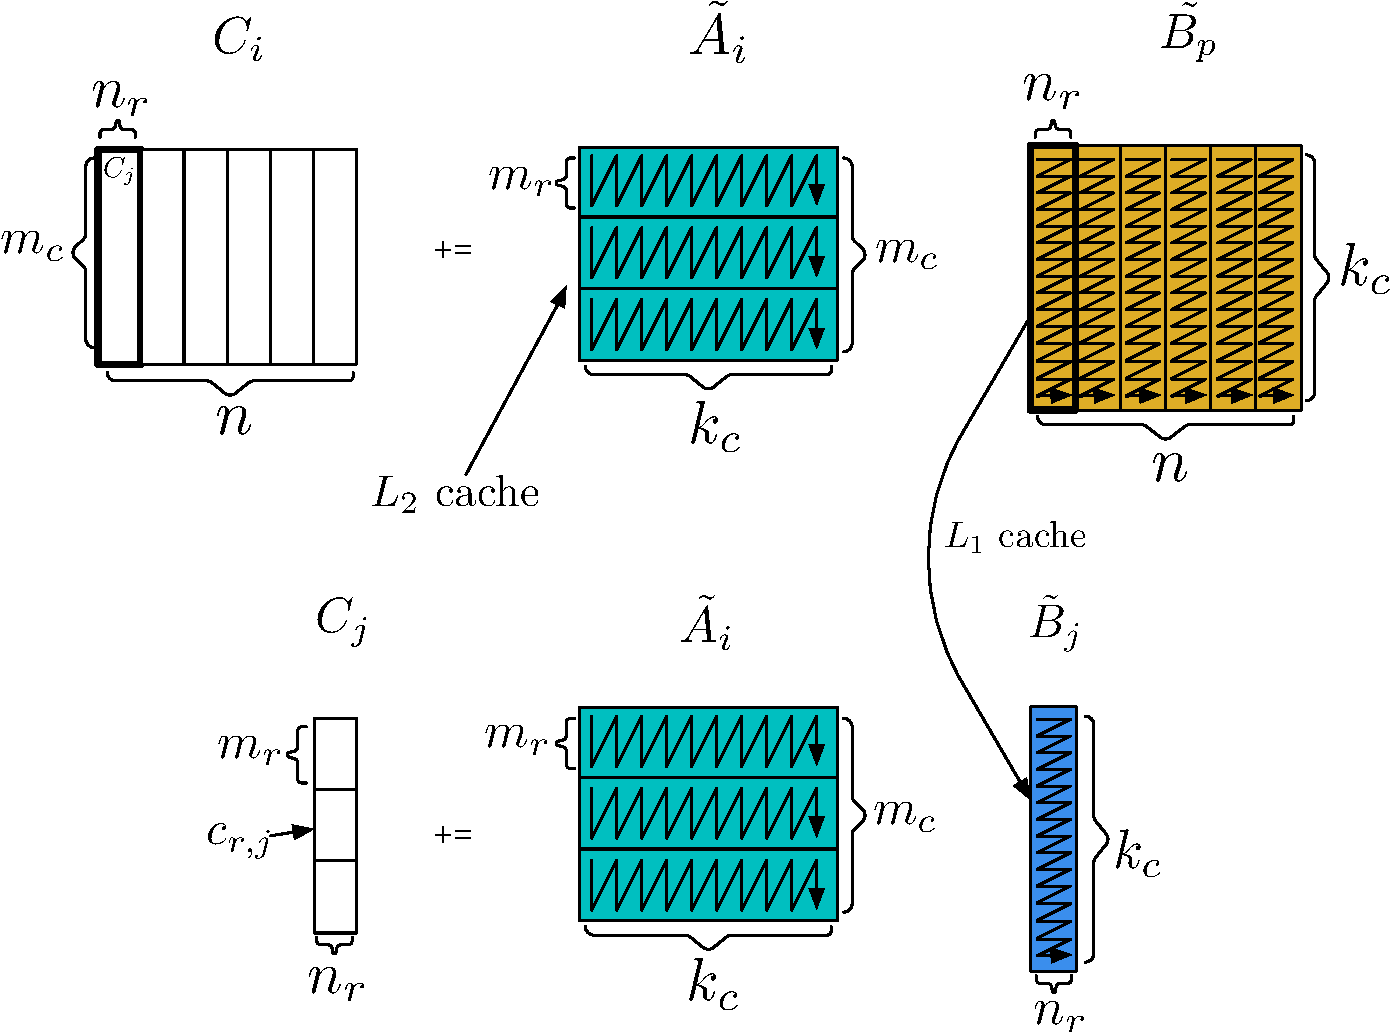
\includegraphics[width=0.95\columnwidth ]{imgs/Goto_second.pdf}
		\caption{Macro-Kernel in the Goto algorithm for Dense Matrix Multiplication (DMM).}
		\label{fig:gotosecond}
\end{figure}



\noindent \textbf{Micro-Kernel}. The micro-kernel is the core operation of blocked matrix multiplication and the speed of the whole routine largely depends on the speed of this kernel. For this reason, in high-performance libraries, the micro-kernel is often written in assembly language, to exploit vectorized instructions and hand-tuned data pre-fetching~\cite{van2015blis}.
The micro kernel computes $c_{r,j} = c_{r,j} + \tilde{A}_j \tilde{B}_j$, where $\tilde{A}_j$ is an horizontal micro-panel of $\tilde{A}_i$ and $\tilde{B}_j$ is a vertical micro-panel of $\tilde{B}_p$, residing, respectively, in L2 and L1 cache, as reported in Figure~\ref{fig:gotothird}. The operation is performed as $k_c$ rank-1 updates, by computing the outer product between a column of  $\tilde{A}_j$ and a row of $\tilde{B}_j$ and by accumulating the results into the $m_r \times n_r$ $c_{r,j}$ submatrix. In this way, $c_{r,j}$ can be kept in CPU registers until the loop over $k_c$ is , allowing to move data from the registers to the memory just once. This means that $2m_c n_c k_r$ FLOPs can be performed with just $m_r n_r$ memory operations. Furthermore, this data reading pattern benefits from the data packing performed in the previous loops. In fact, columns and rows of $\tilde{A}_j$ and $\tilde{B}_j$ respectively will be accessed contiguously, which is generally known to be faster than accessing non-in-stride memory locations~\cite{low2016analytical}. In conclusion, pre-fetching instructions that load successive entries of $\tilde{A}_j$ and $\tilde{B}_j$ are interleaved with instructions performing the rank-1 update. This allows to mask the latency of the caches with the computation time of the CPU.


\noindent \textbf{Choosing the  kernel parameters}. Blocked matrix multiplication requires to determine a number of parameters $n_c, m_c, k_c, n_r, m_r$, controlling how the matrices are gradually decomposed. These parameters can differ from one processor to another, since they are influenced by hardware features such as the cache size or the number of SIMD registers. Choosing the optimal parameters for a given CPU architecture is a research problem, tackled for example by \textit{Low et al. }~\cite{low2016analytical}, which goes beyond the scope of this paper. Here, we want to list some general rules governing good choices for parameters. %We do this to provide a more detailed overview of the  Goto matrix multiplication algorithm. 
The micro-kernel is characterized by $m_r, n_r, k_c$. The values of $m_r$ and $n_r$ should be large enough so that the computation masks the latency of the caches. However, it should also allow to leave space in the registers for the next entries of $\tilde{A}_j$ and $\tilde{B}_j$. $k_c$ should be as large as possible, but must take into account the following constraints: 1) $k_c n_r$ entries from $\tilde{B}_j$ should fit the L1 cache 2) $m_c k_c$ entries from $\tilde{A}_i$ reside in the L2 cache. 
Moreover, cache replacement policies should also be taken into account. These policies control which data are kept and which are discarded from the levels of cache and may impact on the optimal macro-kernel values. A general solution is provided by Goto \textit{et al.}, who suggest choosing $k_c$ so that $\tilde{B}_j$ takes less than the half of the L1 cache~\cite{goto2008anatomy}.

\begin{figure}[t]
	\centering
	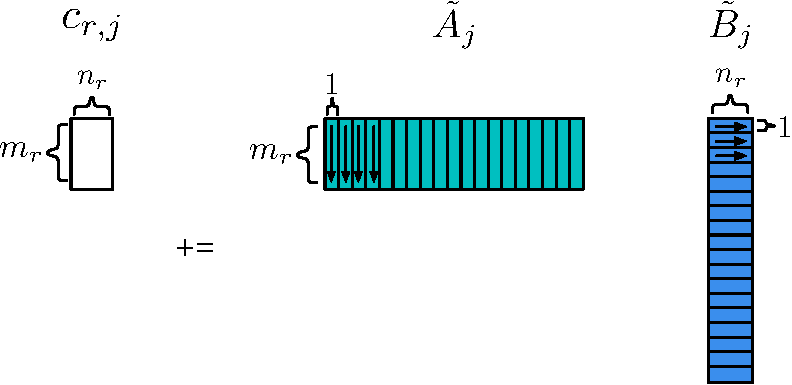
\includegraphics[width=0.8\columnwidth ]{imgs/Goto_third.pdf}
	\caption{Micro-Kernel in the Goto algorithm for Dense Matrix Multiplication (DMM).}
	\label{fig:gotothird}
\end{figure}

% The correct choice of these parameters
%strictly depends on the underlying hardware features.
%In the original work, Goto \textit{et al.} suggest to choose $k_c$ so that $\tilde{B}_j$ takes less of the half of the L1 cache~\cite{goto2008anatomy}. Cache replacement policies should also be taken into account. These policies control which data are kept and which are discarded from the levels of cache and may impact on the optimal macro-kernel values. \cosimo{This involves deep architectural fe}
% This is a non-trivial architecture-dependent problem which goes beyond the scope of this article.
%%\fnote{frase sopra. proverei a scriverla meglio spiegando perche' non la addressiamo. sembra che sia difficile e quindi ci importa una sega :)}
%
%Cache replacement policies should also be taken into account, especially in the $\tilde{B}_j$ case~\cite{goto2008anatomy,low2016analytical}, giving birth to a non-trivial architecture-dependent problem which goes beyond the scope of this article.
%\fnote{frase sopra non capisco. piu' chiara...}
Concerning the macro-kernel, we already discussed that the $m_c k_c$ product should be as large as possible. One of the key insights of the Goto algorithm is to consider the role of the Translation Look-Aside Buffer (TLB) in choosing the macro-kernel parameters. To hide the limits of random-access memories capacity (RAM), modern computing architectures use virtual memory. With this mechanism, the memory (RAM and hard disk) is partitioned into pages and a table, called \textit{page table}, keeps track whether a page is in memory or on disk. Scanning the page table entails additional overhead to check whether the requested page is on memory or disk.
Hence, the TLB, which is smaller than the overall \textit{page table}, keeps track of the most recently used pages: in case of a TLB \textit{hit}, the translation is fast. On the other side, in case of a TLB \emph{miss}, the complete \textit{page table} is checked and the new entry is moved to the TLB. Actually, the TLB has the same role as the cache and the \textit{hit/miss} dichotomy involves the same consequences. Thus, besides ensuring that $m_c k_c$ entries from $\tilde{A}_i$ fit the L2 cache, it is crucial that $\tilde{A}_i$, $n_r$ columns from $C_k$, and $n_r$ columns of $\tilde{B}_j$ are simultaneously addressable by the TLB, to avoid TLB misses during the block-panel multiplications of the macro-kernel. The only limit to the $n_c$ parameter is that $k_c n_c$ have to fit the L3 cache.

\subsection{Dense Neural Forward Pass Time Predictor}
\label{subsec:densetimepred}
In the previous section, we detail how Dense Matrix Multiplication is implemented on modern CPU architectures. We now show how the insights deriving from a deep understanding of matrix multiplication can be used to develop a time predictor for a Feed Forward Network (FFN) forward pass. We empirically demonstrate that even the highly engineered Goto algorithm  suffers when dealing with edge matrix dimensions. Hence, we leverage this intuition to build a hybrid analytical-empirical model for predicting dense matrix multiplication.
A FFN is composed of a  stack of \textit{fully connected} layers, where each neuron of layer $i$ is connected to all neurons of layer $i+1$. Each layer is composed of a weight matrix $W_i$, a bias vector $b_i$ and a non-linear \textit{activation function} $\sigma_i( \cdot )$. Let $x_i$ be the input to the $i$-th layer, the forward pass of layer $i$ is described by:
\begin{equation}
	\label{eq:mlpforward}
	x_{i+1} = \sigma_i(W^t_i x_i + b_i)
\end{equation}
where $x_{i+1}$ represents the output of the $i$-th layer. 
Hence, forwarding through a FFN layer consists of: 1) multiplying the input with the weight matrix, 2) summing the bias, 3) applying a non-linear activation function, usually ReLU or its variants. The overall forward pass on a FFN of $d$ layers has a cost, in terms of execution time, given by:
\begin{align}
 \label{eq:overallcost}
 	T = t_m \cdot ( f \cdot l_1 + \sum_{i=2}^{d} l_i   l_{i-1} + l_{d})
 	 + t_a \cdot \sum_{i=1}^{d} l_i + t_r \cdot \sum_{i=1}^{d} l_i \nonumber \\
 	   \simeq t_m \cdot ( f \cdot l_1 + \sum_{i=2}^{d} l_i \cdot  l_{i-1} + l_d) 
 \end{align}
where $t_m $ is the normalized time per multiplication, $t_a$ is the time for addition, $t_r$ is the time to perform the ReLU operation on a single neuron. As reported in Equation~\ref{eq:overallcost}, the time to perform matrix multiplication dominates the overall execution time, both in terms of number of operations and in terms of the complexity of the operation itself. We observe that $t_m$ can be inferred as:

\begin{equation}
	\label{eq:tm}
	t_m = \frac{1}{\text{GFLOPS}}
\end{equation}
The theoretical peak of GLOPs can be derived form the hardware specifications of the processor\footnote{https://software.intel.com/en-us/articles/a-simple-example-to-measure-the-performance-of-an-intel-mkl-function}. However, real performance can be significantly different from the theoretical ones, especially when facing limit cases, such as narrow or wide matrices. To include these cases into our evaluation, we develop a prediction model to measure the performance of a specific neural networks architecture.

Among the different instantiations of the BLAS library, we choose \textit{oneDNN}\footnote{\url{https://github.com/oneapi-src/oneDNN}},
a C++ high-performance framework for deep learning primitives developed by Intel, used as backbone inference system by Pytorch~\cite{NEURIPS2019_9015}, Tensorflow~\cite{abadi2016tensorflow}. With respect to the Math Kernel Library (MKL)~\cite{wang2014intel} by Intel, oneDNN guarantees the same performances while being open source.
The oneDNN library adopts the following parameters for CPUs with AVX2 ISA enabled: $m_c = 10000$, $n_c =384 $, $k_c = 192$, while for the micro-kernel we have  $m_r = 24, n_r = 4$.
%---------------- BEGIN MKL DETAILS----------------------
% Before moving on the empirical GFLOPs estimation, we analyze some of the features of the oneDNN library. 
% OneDNN adopts the following  parameters for CPUs with AVX2 ISA enabled: $m_c = 10000$, $n_c =384 $, $k_c = 192$, while for the micro-kernel we have  $m_r = 24, n_r = 4$.
The macro-kernel parameters $m_c, n_c, k_c$  are selected to deal with very large matrices; for the sequential case, the library contains a mechanism to tailor smaller shapes. Let us call $\overline{m}_c$, $\overline{n}_c$, $\overline{k}_c$ the parameters that the macro and micro kernels actually use. 	
$\overline{m}_c$ is chosen as:
$$\overline{m}_c = \texttt{rnd\_up}(min(max(m, m_r), m_c
), m_r)$$
%\fnote{sopra ho messo textt la chiamata a procedura. ti piace? se si, fixa everywhere. FM}
where \texttt{rnd\_up}($a,b$) is a function which approximates $a$ as $a = n^{*} b$, with $n^{*} = min\{n \ |\  nb \geq a\}$, \textit{i.e.}, to the subsequent multiple of $b$. This way, it is ensured that $\overline{m}_c$ is larger than the micro-kernel parameter $m_r$ and that the default $m_c$ is not involved if $m \leq m_c$. By means of the \texttt{rnd\_up} function, we ensure that $\overline{m}_c \bmod m_r  = 0$ to avoid undersized horizontal $\tilde{A}_j$ panels in the micro-kernel.  
%When the resulting $m_c > m$,  we pad with zeros the difference $d = m_r - m$. This means that $d$ values are read and written but they are not actually used, causing a performance drop.
Similar refinements are adopted to chose $\overline{n}_c$ and $\overline{k}_c$. Moreover, oneDNN triggers when the cost of packing the matrices into contiguous arrays surpasses the cost of multiplication. In this case, besides changing the macro-kernel parameters, it also performs a different routine that skips copying the matrices in cache-aware buffers.

%In choosing $\overline{k}_c$, oneDNN introduces two parameters  $k_{ct} = 256$, which stands for $k_c$ traditional, and $k_{cs}$, for $k_c$ small. $\overline{k}_c$ is computed as function of the shared dimension $k$ as:

% \begin{algorithm}
% 	%	\KwData{this text}
% 	%	\KwResult{how to write algorithm etith \LaTeX2e }
% 	$\overline{k}_c$
% 	\uIf{$k < k_{ct}$ }{
% 		$\overline{k}_c = max(128 , \overline{k}_c)$\;
% 	}\uElseIf{$k < 2 k_c$ }{
% 		$\overline{k}_c = (k+1)/2)$\;
% 	}\Else{
% 		$\overline{k}_c = k_c$\;
% 		}
% \end{algorithm}
% The actual value of the blocking parameter $n_c$, namely $\overline{m}_c$ is chosen depending on both $n_c$ and $k_c$. One more parameter is introduced, $n_{csk}$ which is used when $\overline{k}_c$ is small.

% \begin{algorithm}
% 	$\overline{m}_c = (k<k_{cs}) ? n_{csk} : n_c $\;
% 	$\overline{m}_c = rnd\_up(min(max(n, n_r), n_c), n_r)$	\;
% \end{algorithm}

% Furthermore, oneDNN triggers when the cost of packing the matrices into contiguous arrays surpasses the cost of multiplication. In this case, besides changing the macro-kernel parameters, it also perform a different routine that skips copying the matrices in cache-aware buffers.
%---------------- END MKL DETAILS----------------------

In Section~\ref{subsec:dmm} we have described the optimization techniques beyond Dense Matrix Multiplication on modern CPUs. We also detail the tailored refinements implemented by the oneDNN framework to deal with matrices where at least one dimension is small. We now show the performance of the oneDNN framework with differently shaped matrices, aiming at identifying a reliable $t_m$ for Equation~\ref{eq:tm}. In these experiments, we multiply random matrices with different shapes to empirically analyze how the oneDNN library adapts to different matrix dimensions. We propose two different cases: 1) $m=k$, 2) $mk=c$, with $c$ as a constant integer.
We run our tests on a i9-9900K processor, with AVX2 instructions, 3.6 GHz, max frequency 5.0 GHz. Each core has a 32 KiB L1 cache for data, 32 KiB L2 cache for instructions, both 8-way set associative, 256 KiB L2 cache 4-way set associative, and 2 MiB L3 cache, 16-way set associative. We report the results for single-thread execution. 
In our first experiment, we vary $m$ and $k$ in a fixed range and report the corresponding GFLOPs, with different values of $n$. Observe that $A$, of shape $m \times k$,  represents the weight matrix $W$, $B$, of shape $k \times n$ represents the input matrix $x$, obtained by stacking $n$ input vector. We vary $m$, $k$ and $n$ to model real use-case scenarios: $m$ and $k$ correspond to the sizes of Feed Forward Network layers, while $n$, the \emph{batch size}, is the number of documents we give in input to the neural network at a time. Results are reported in Figure~\ref{fig:onednnl_no_r}, which shows that GFLOPS grow as the size of the matrices even with the aforementioned techniques tailored to edge cases. In Figure~\ref{fig:onednnl_rev}, we show the results of the reverse experiment: instead of gradually increasing both $m$ and $k$, we keep the size of $A$ constant (the $mk$ product is constant). The figure shows that small values of $m$ with large values of $k$ still afford  high-performance (left side of the graph). On the other hand, small values of $k$ paired with larger values of $m$ cause serious performance degradation. The variation of the GFLOPS with the matrix shapes suggests that a unique and size-independent $t_m$ is not reliable. As aforementioned, this evidence some limitations of the Goto algorithm when dealing with edge combinations of input dimensions.
A correct analysis expresses $t_m$ as a function of the $m,n,k$ parameters, or in the case of the Feed Forward Network , as a function of the dimensions of the layers, \textit{i.e.}, $t_m = t_m( l_1, \dots, l_{d})$.
Given the variability of the performance with input shapes, we shall empirically measure them.
 We can use Figure~\ref{fig:onednnl_no_r} and ~\ref{fig:onednnl_rev} to derive a lookup table that maps the matrix shapes to the corresponding GFLOPs. The previous graphs are synthesized in Figure~\ref{fig:heatmap}, which shows an heatmap of the GLFOPs with different values of $m$ and $k$ and $n = 1000$.

 We observe three performance zones, defined by horizontal stripes induced by partitioning the $k$ axis.
\begin{itemize}
	\item $K \geq 512$ : high-performance (130 GFLOPs)
	\item $128 \leq K \leq 512$: Medium performance (110 GFLOPS)
	\item $K \leq 128$: Low performance (90 GFLOPs)
\end{itemize}



% \begin{figure}
% \begin{minipage}[b]{\columnwidth}
% 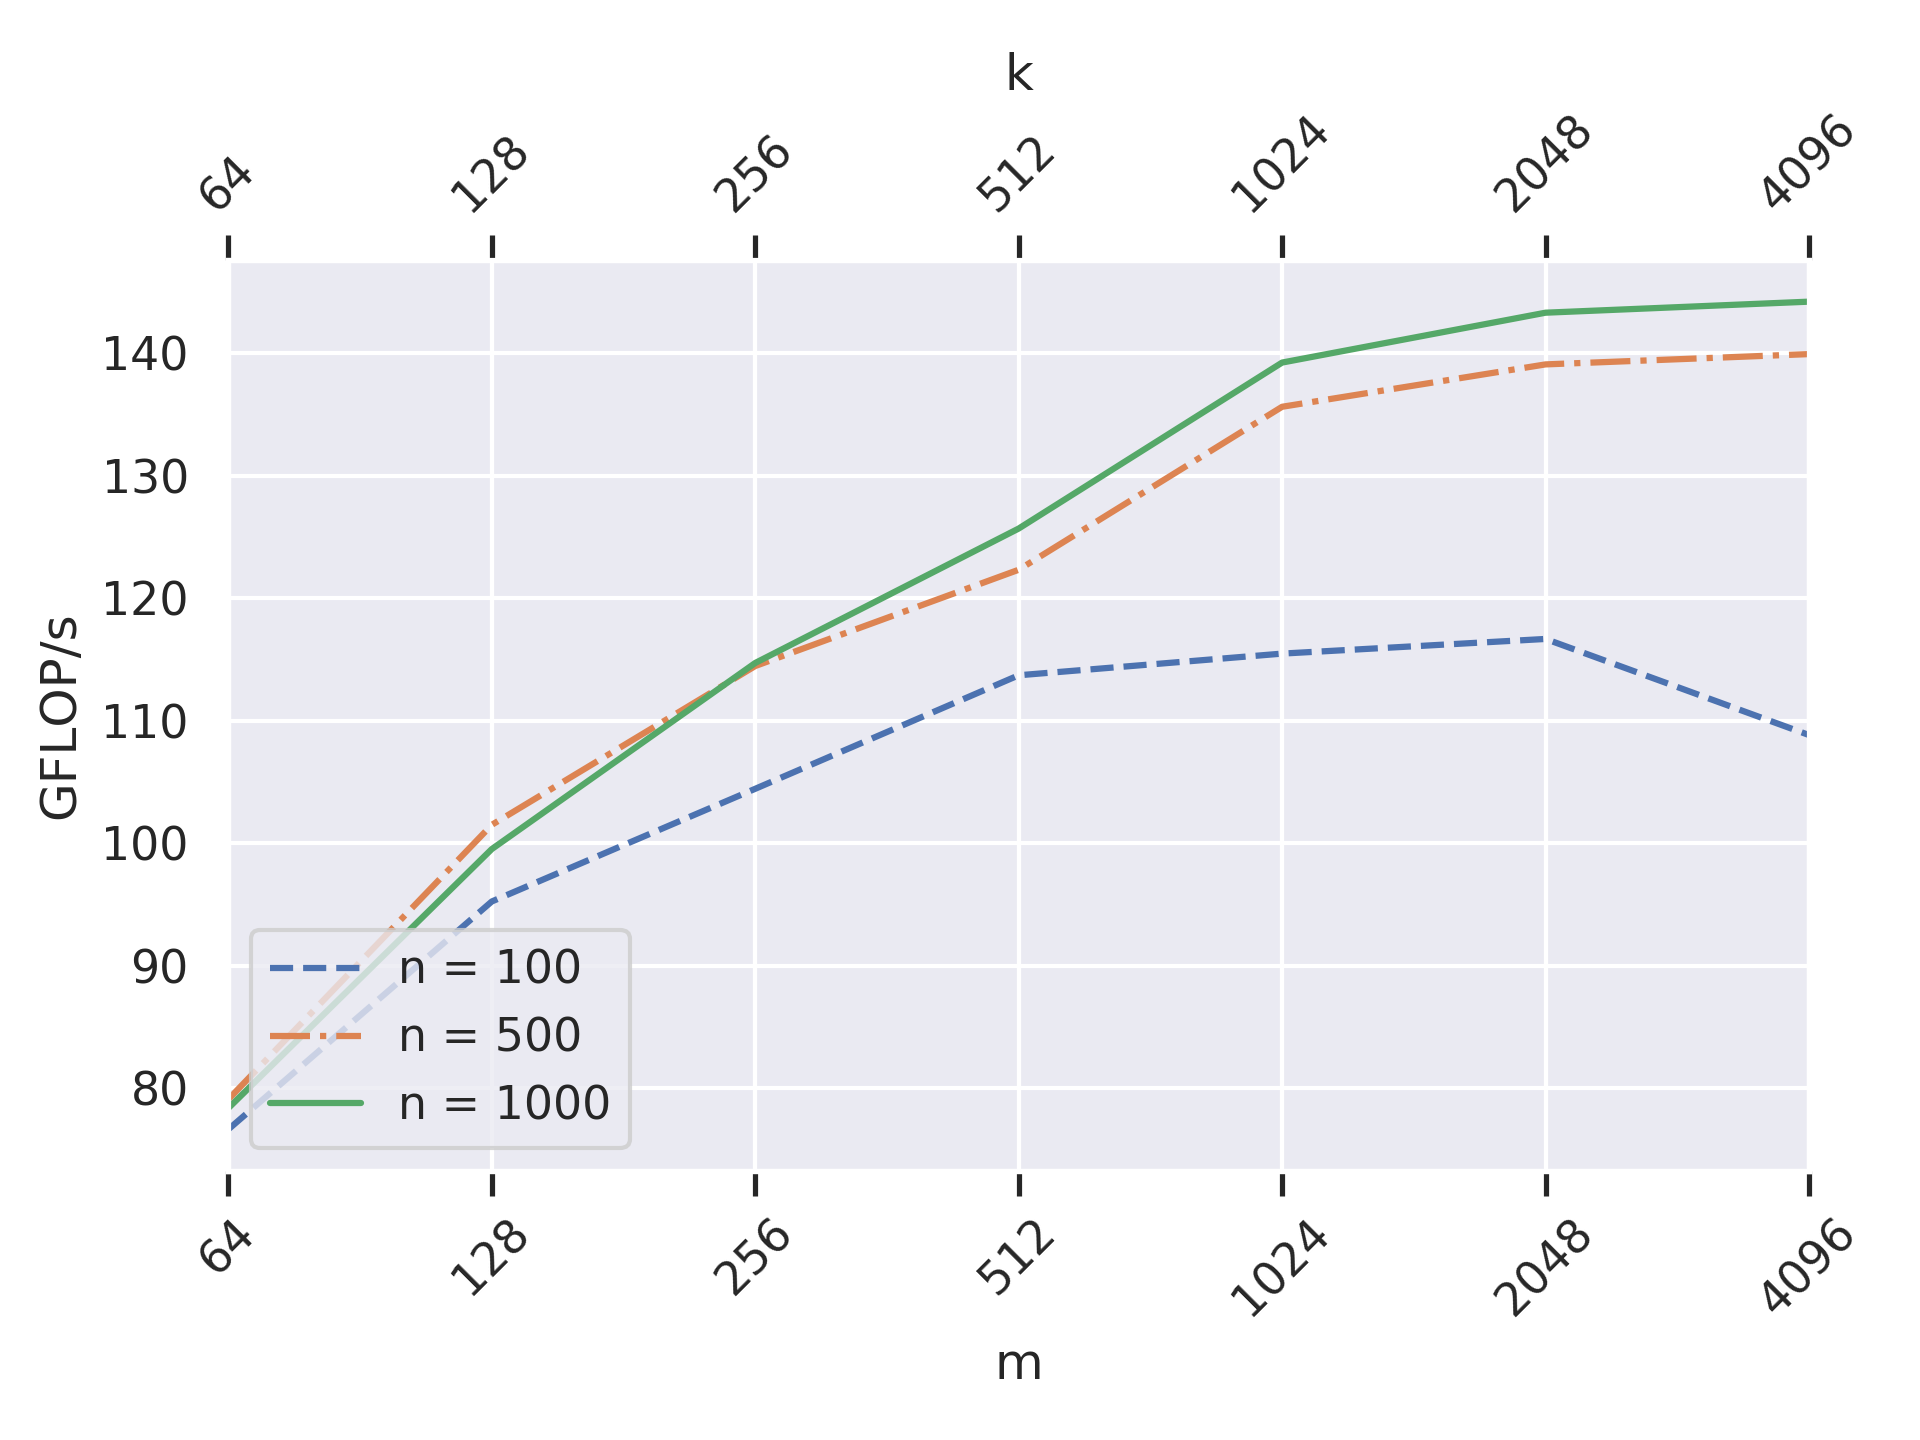
\includegraphics[width=\columnwidth]{imgs/DNNL_different_N.png}
% %\centering 
% %\caption*{Static}
% \end{minipage}%
% \\ 
% \begin{minipage}[b]{0.5\columnwidth}
% 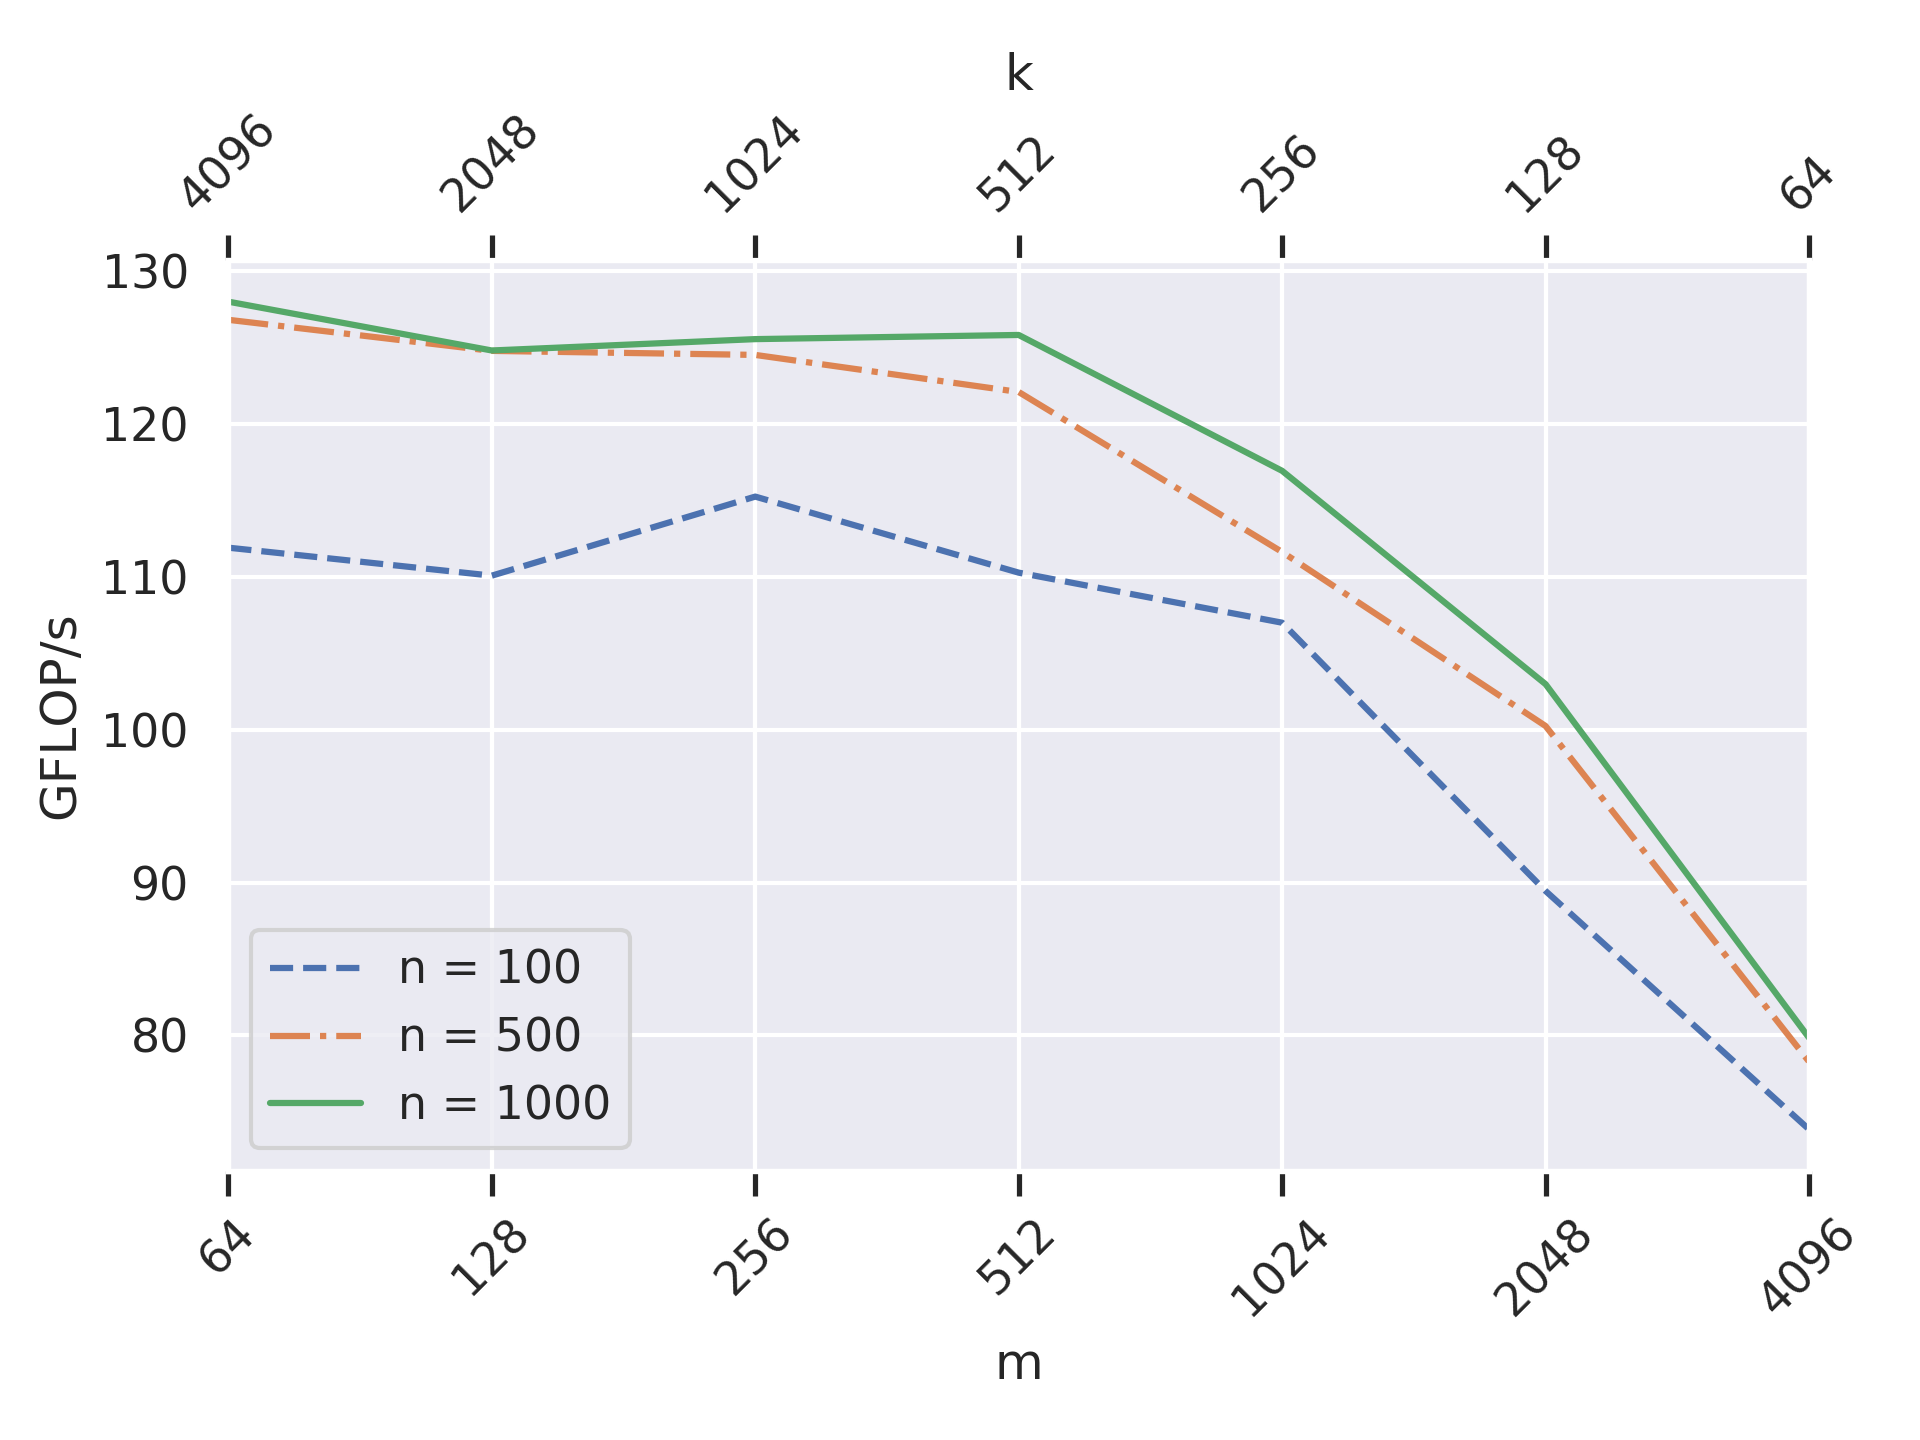
\includegraphics[width=\columnwidth]{imgs/DNNL_different_N_reverse.png}
% %\centering 
% %\caption*{Dynamic}
% %\subcaption{Another subfigure}
% \end{minipage}%
% \caption{Matrix Multiplication with oneDNNL}
% \label{fig:onednnl}
% \end{figure}

\begin{figure}	
	\centering
	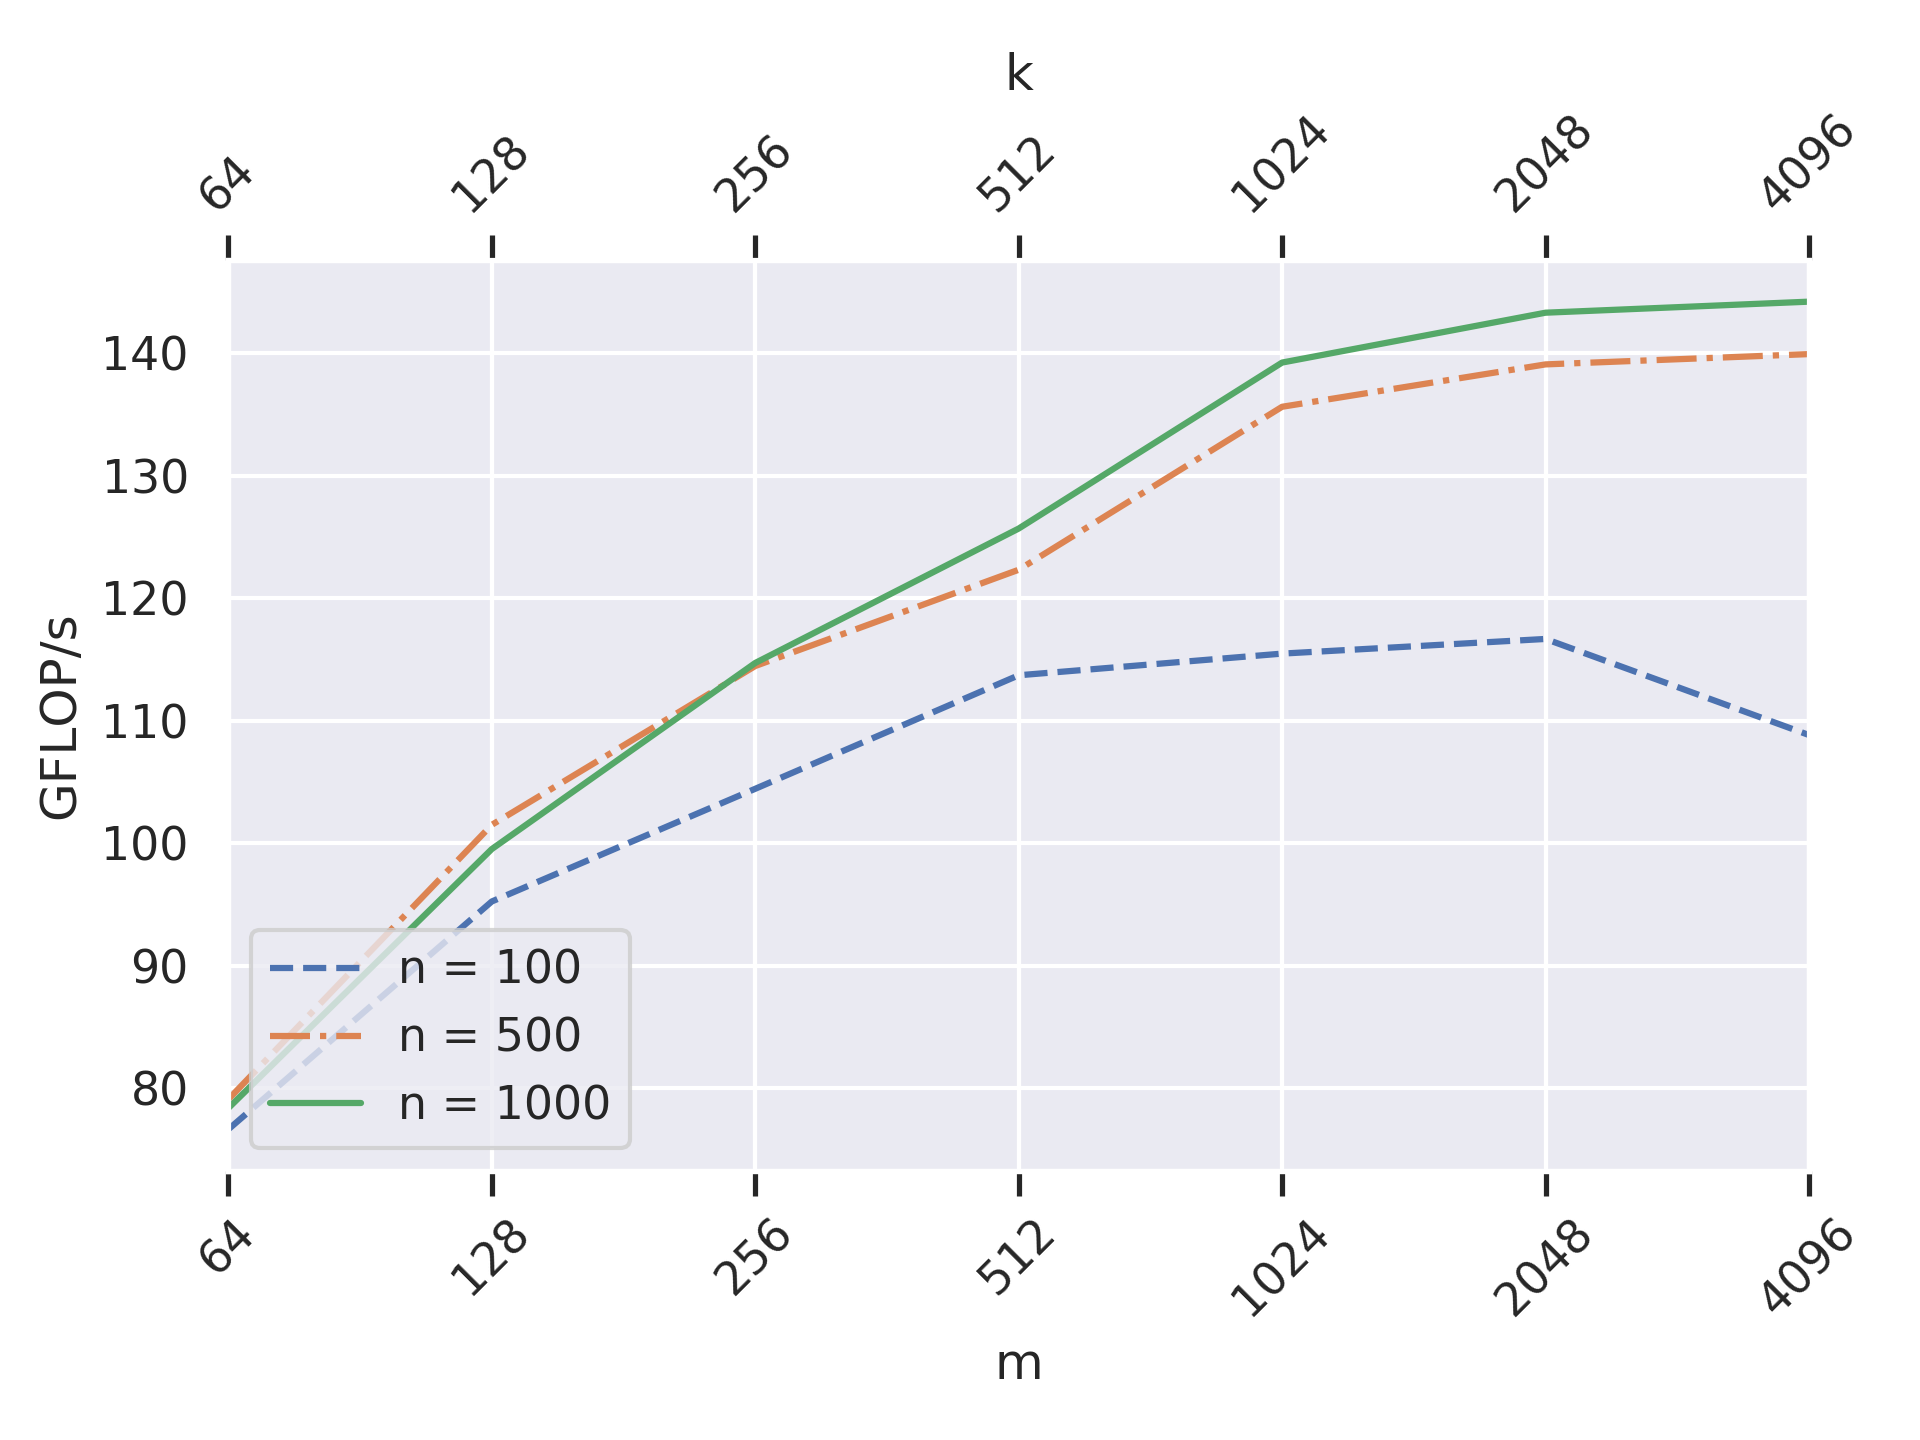
\includegraphics[width=\columnwidth]{imgs/DNNL_different_N.png}
	\caption{Matrix Multiplication with oneDNN, as $m$ and $k$ grow.  }
	\label{fig:onednnl_no_r}
\end{figure}

\begin{figure}
	\centering
	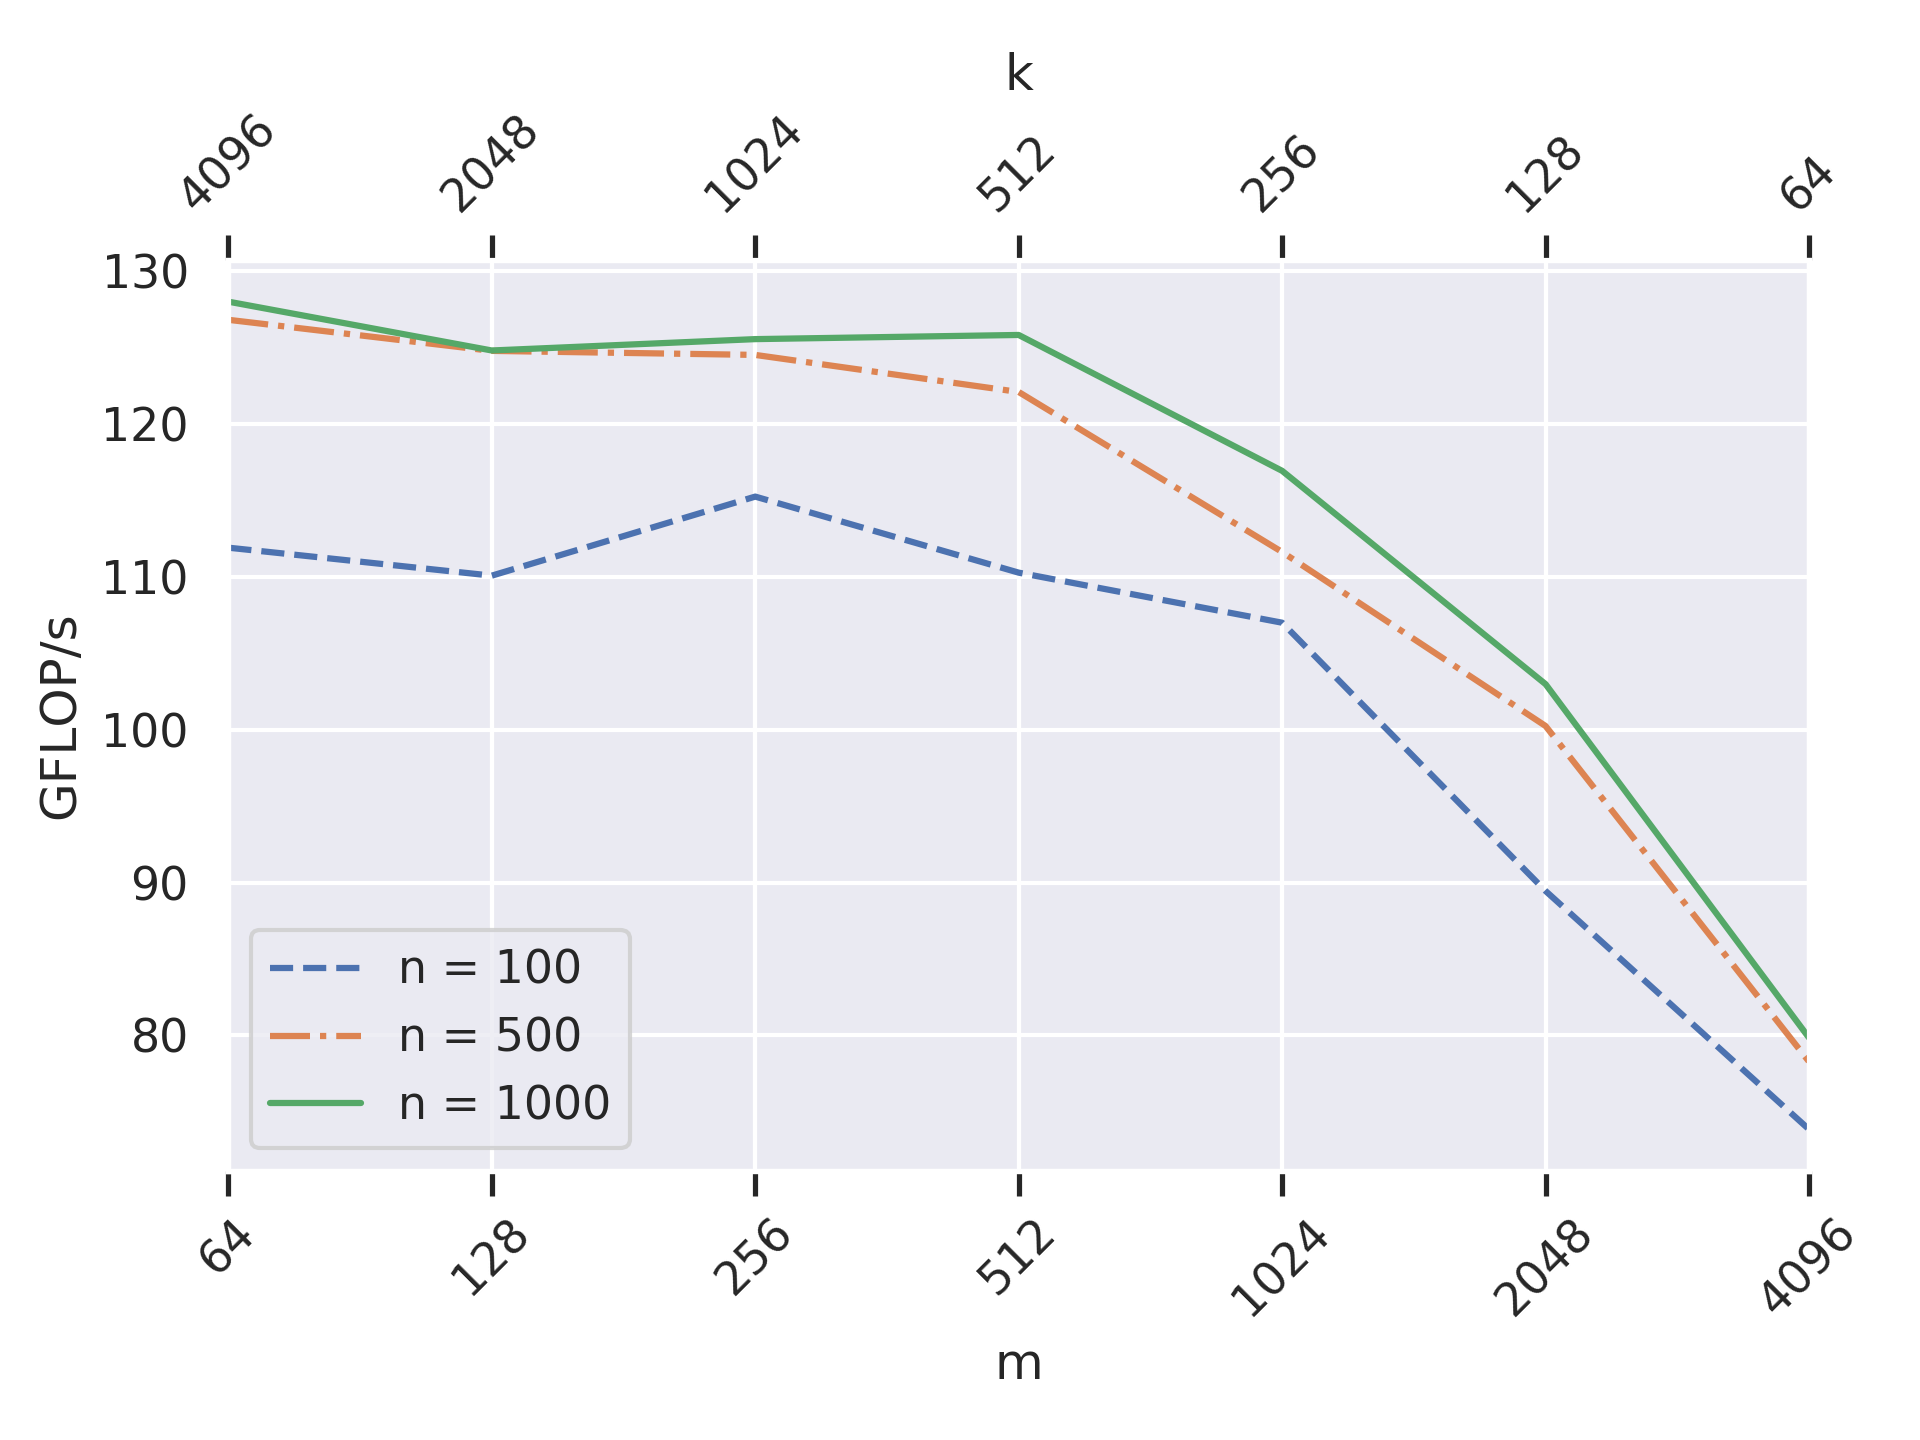
\includegraphics[width=0.8\columnwidth]{imgs/DNNL_different_N_reverse.png}
	\caption{Matrix Multiplication with oneDNN, with the product $mk$ constant. }
	
	\label{fig:onednnl_rev}
\end{figure}

\begin{figure}
	\centering
	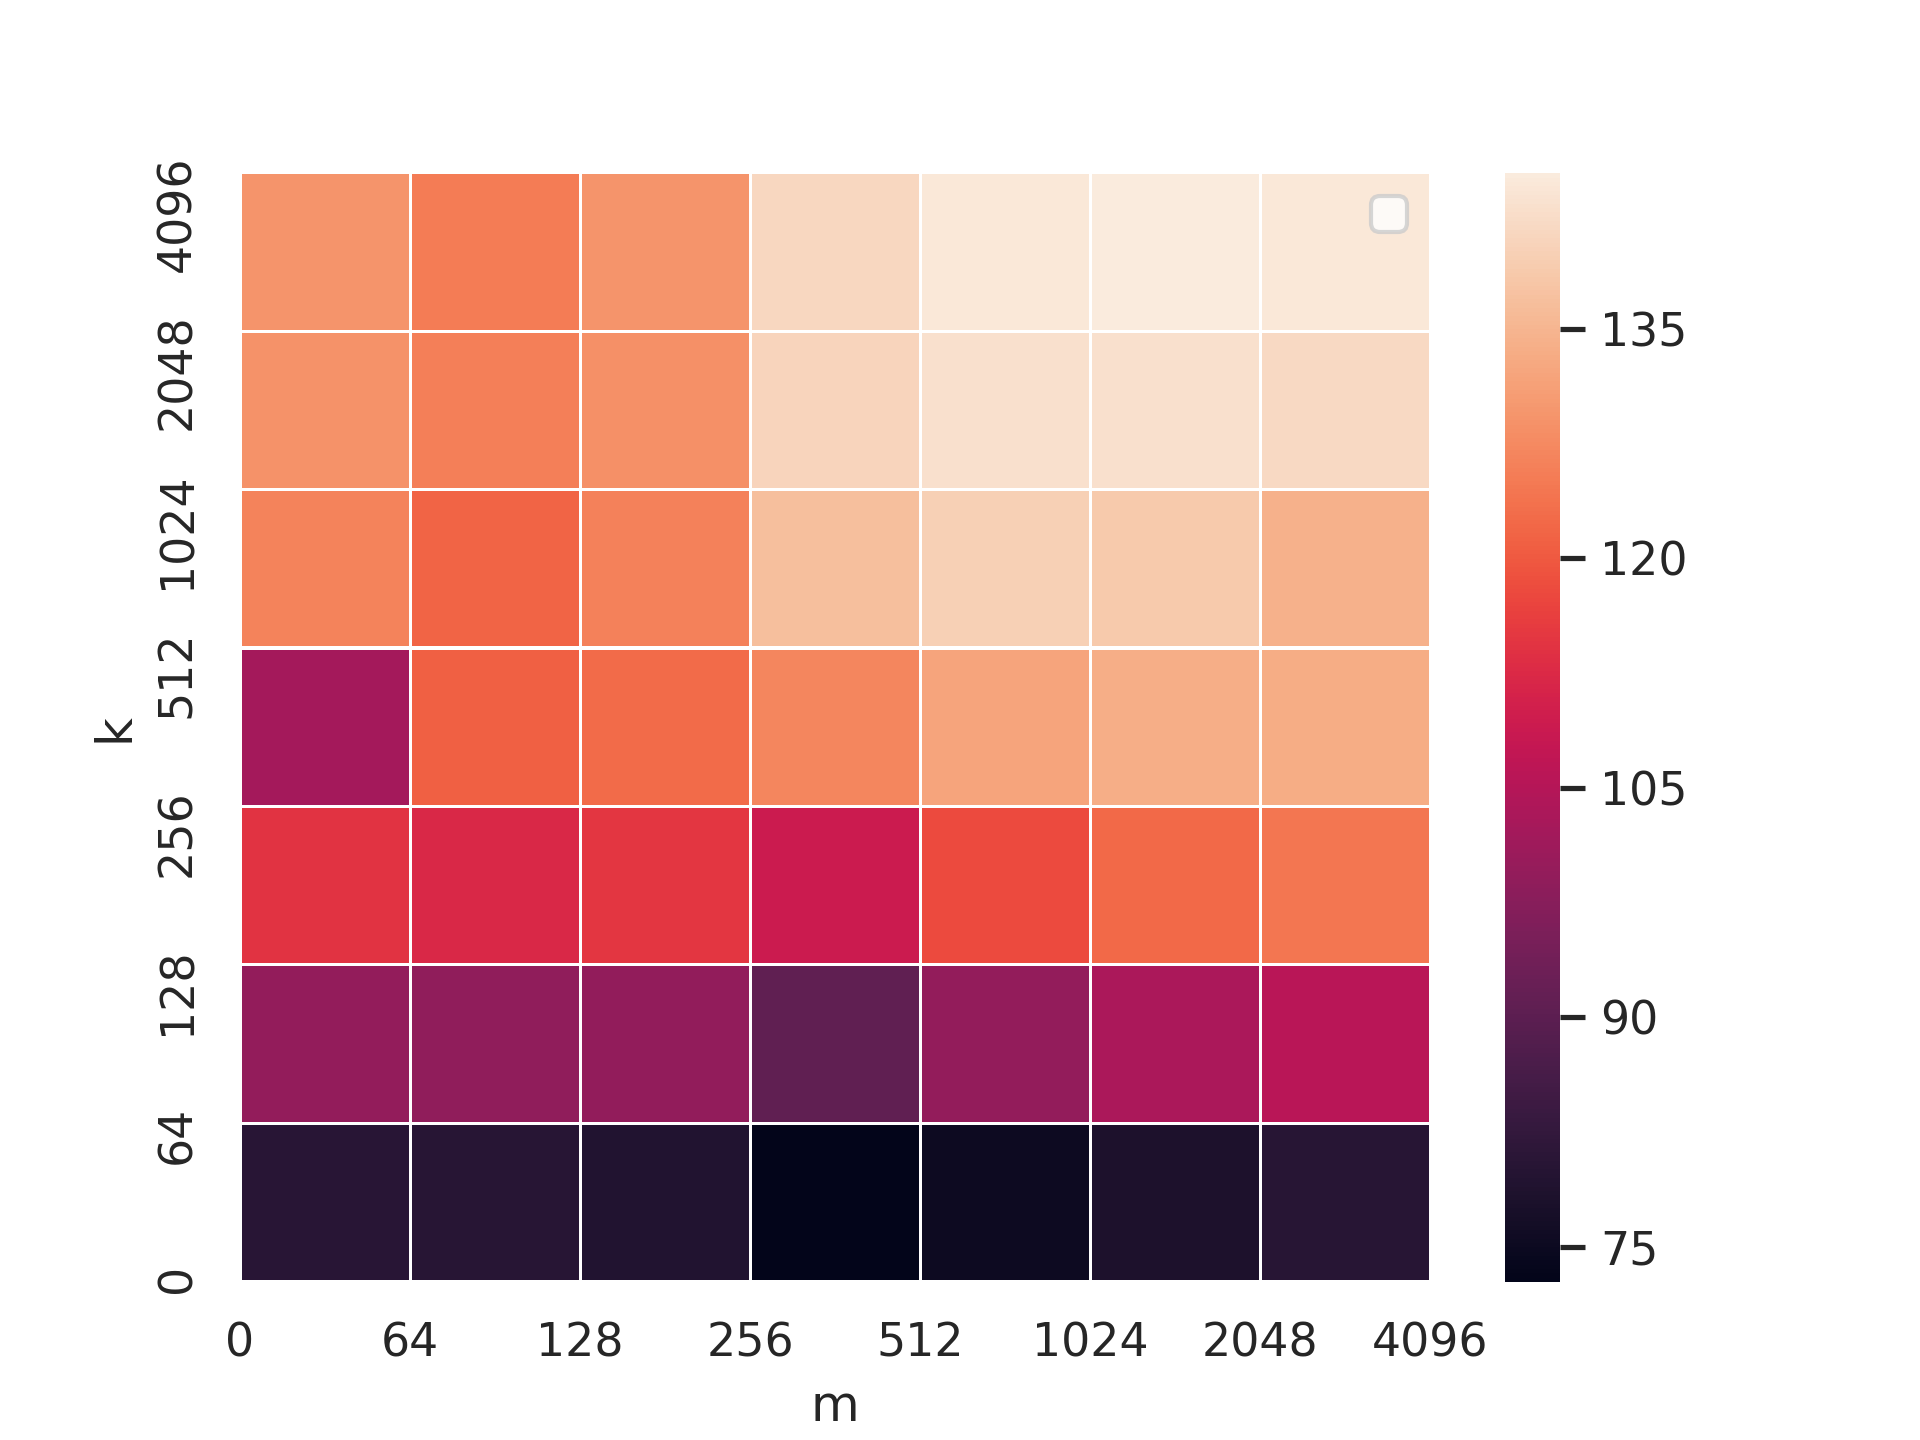
\includegraphics[width=\columnwidth]{imgs/heatmap_gflops_batch1000.png}
	\caption{Matrix Multiplication HeatMap with n = 1000.}
	\label{fig:heatmap}
\end{figure}


For a network of size $\{1000, 500, 500, 100 \}$, we can assume to be always in the high-performance region, except for the last layer. Observe that the last layer has a negligible impact on the overall forward time and we can ignore it. Table~\ref{table:est_vs_real_exec_t} illustrates how the prediction model can substitute the experimental procedure of training and testing a model, turning out to be essential to reduce the architecture search space.

\begin{table}[htb]
	\centering

	%\adjustbox{max width=\columnwidth}{
	\begin{tabular}{lrr}
	%\resizebox{\columnwidth}{!}{
		\toprule
		\multirow{2}{*}{Model} &    \multicolumn{2}{c}{Scoring Time ($\mu s$/doc)} \\
		\cmidrule{2-3}
		 & Real & Predicted \\		%    \thead{Real Scoring & \\ Time per doc ($\mu s $)}  & \thead{Real Scoring & \\ Time per doc ($\mu s $)} \\
		\midrule

		 1000$\times$500$\times$500$\times$100 & 14.4& 14.5 \\
		 200$\times$100$\times$100$\times$50 & 	1.3& 1.3 \\
		 300$\times$150$\times$150$\times$30 & 2.0 & 2.2 \\
		 500$\times$100 & 2.1 & 2.2\\
 		\bottomrule
	\end{tabular}
	 %}
	\caption{Performance of our dense prediction model. Real execution times measured with batch size = 1000.}
	\label{table:est_vs_real_exec_t}
\end{table}

\subsection{Sparse-Dense Matrix Multiplication} 
\label{subsec:sdmm}
In this section, we study Sparse-Dense Matrix Multiplication (SDMM), a special case of matrix multiplication where the first matrix is \textit{sparse}: we recall that \textit{sparsity} is defined as the percentage of zero entries in a data structure, in this case, a matrix. First, we describe a common format to store sparse matrix, \textit{Compressed Sparse Row} (CR). Then, we detail how SDMM is implemented on modern CPU processors. 

\smallskip
\noindent \textbf{CSR Format}.
A sparse matrix is completely identified by its non-zero values and their positions since all the others entries are zeros. This motivates the use of a different representation for sparse matrices w.r.t. to dense ones. The different representation aims at saving storage space and improving the performance of matrix multiplication. For this purpose, several formats have been developed: the most common are Compressed Sparse Row (CSR), Compressed Sparse Column (CSC), Coordinate List (COO). Among them, we analyze CSR, since it is usually supported by off-the-shelf libraries, both for storing and for matrix operators, such as multiplication and it naturally fits to Sparse-Dense Matrix Multiplication, as we will detail.
%Let us assume we have a matrix $A \in \mathcal{R}^{m \times k}$ with $nnz$ non-zero values.
%$$ \text{sparsity} = \frac{nnz}{mk}$$

Let us consider a matrix $M \in \mathbb{R}^{m \times n}$ with $nnz$ non-zero elements. 
An example of the  CSR representation is reported in Figure~\ref{fig:sparsecsr}. It consists of three vectors: \textit{values} $\in \mathbb{R}^{nnz}$, \textit{columnIndex} $ \in \mathbb{R}^{nnz}$, \textit{rows} $\in \mathbb{R}^{m+1}$. 
The \textit{values} array stores the non-zero entries, and \textit{columnIndex} stores their column index in the original matrix, meaning that \textit{columnIndex}$[i]$ stores the columns index of \textit{values}$[i]$. The \textit{rows} array is built so that $rows[i+1] - rows[i] $ is the number of non-zero entries for row $i$. 

\begin{figure}
\centering
	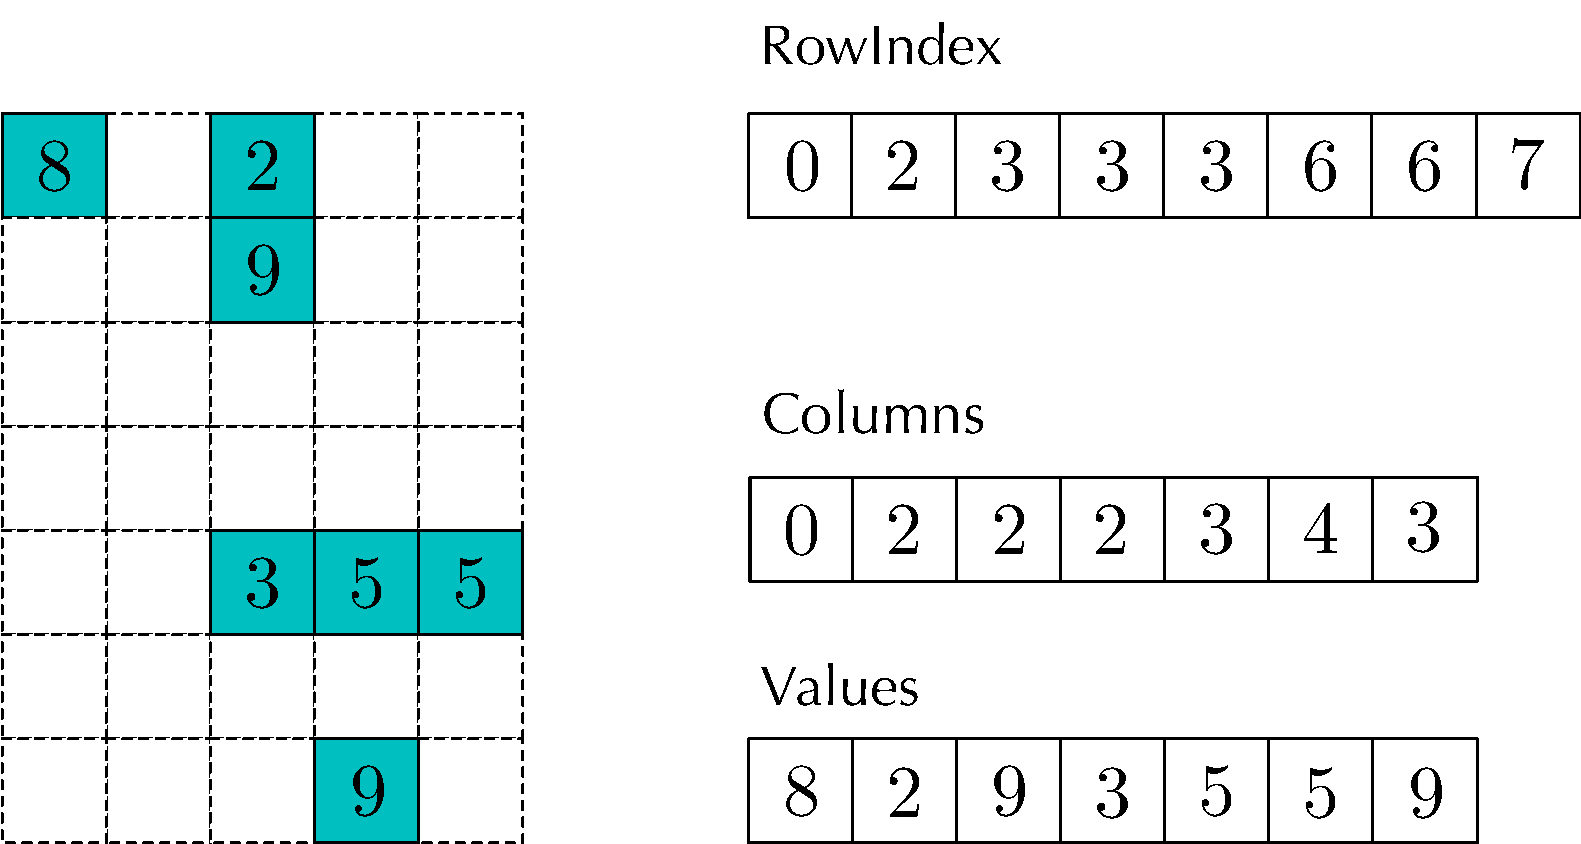
\includegraphics[width=0.8\columnwidth]{imgs/CSR_sparse.pdf}
	\caption{CSR Format for Sparse Matrices.}
	\label{fig:sparsecsr}
\end{figure}


\smallskip
\noindent \textbf{Sparse Dense Matrix Multiplication}.
Sparse Dense Matrix Multiplication or sparse Multi-vector multiplication (SDMM) has a large range of applications: fluid dynamics, graph analysis~\cite{tiskin2001all}, non-negative matrix factorization~\cite{kim2011fast}, economic modeling, seismic simulations~\cite{breuer2019petaflop}, and machine learning~\cite{NIPS2010_4099}. Pruning a neural network pre-trained model naturally induces the usage of SDMM in the forward pass of a Multi-Layer Perceptron, since it converts dense weights into sparse ones. Let us consider Equation~\ref{eq:mlpforward}: in the most general case $W$ represents the dense weight matrix. After pruning, $W$ is transformed into a sparse matrix $\dot{W}$, thus converting $\dot{W}^T x$  into a Sparse Dense Matrix Multiplication.
%Historically, the scientific community has mainly focused in optimizing the Sparse Matrix dense vector multiplication (SpMV). Even if SpMM can be implemented as a loop of SpMV, this approach fails in exploiting data locality in the sparse matrix~\cite{zheng2016semi}. 

%Before describing cutting-edge implementations	 of SDMM, we depict the na\"ive algorithm induced by the CSR Format. %repparse matrix multiplication is slowed down by random memory accesses. Several approaches create their own matrix format to reduce this drawback, even exploiting domain-specific knowledge to guess information on the structure of the matrix. In our case, the structure of the matrix is known \textit{ a priori} but has no specific structure since it derives from the pruning of a neural network. 
Consider the operation $C = AB$, where $A \in \mathbb{R}^{m \times k}$ is a sparse matrix in the CSR representation with $nnz$ non-zero values, and $B \in \mathbb{R}^{k \times n}$, $C \in \mathbb{R}^{m \times n}$ are dense matrices. 
The mundane algorithm induced by A being in CSR Format is reported in Algorithm~\ref{alg:csr_mult}. This format is suitable for row-wise access, allowing to consider exclusively the non-zero entries of the left-side matrix. 
The total number of floating-point operations is reduced from $2mnk$ to $2 nnz N$ w.r.t. dense case, but the irregular access pattern induced by sparsity hinders the efficiency of the algorithm. To overcome this problem, a twofold strategy, as for the dense case, is applied: 1) proficient data access pattern, 2) optimization of the core operation (\textit{micro-kernel}). 

The most used library for sparse matrix multiplication is the Math Kernel Library (MKL)~\cite{wang2014intel}, which implements the sparse versions of third level BLAS routines. Since the library is closed and there are no details on how the multiplication is implemented\footnote{https://community.intel.com/t5/Intel-oneAPI-Math-Kernel-Library/Sparse-Dense-Matrix-Multiplication/m-p/1173953}, we refer to the implementation of the LIBXSMM~\cite{heinecke2016libxsmm}, which is open-source. Later on in this section, we show that LIBXSMM actually outperforms MKL in the spectrum of shapes involved by our neural networks. 

\begin{figure}
\centering
	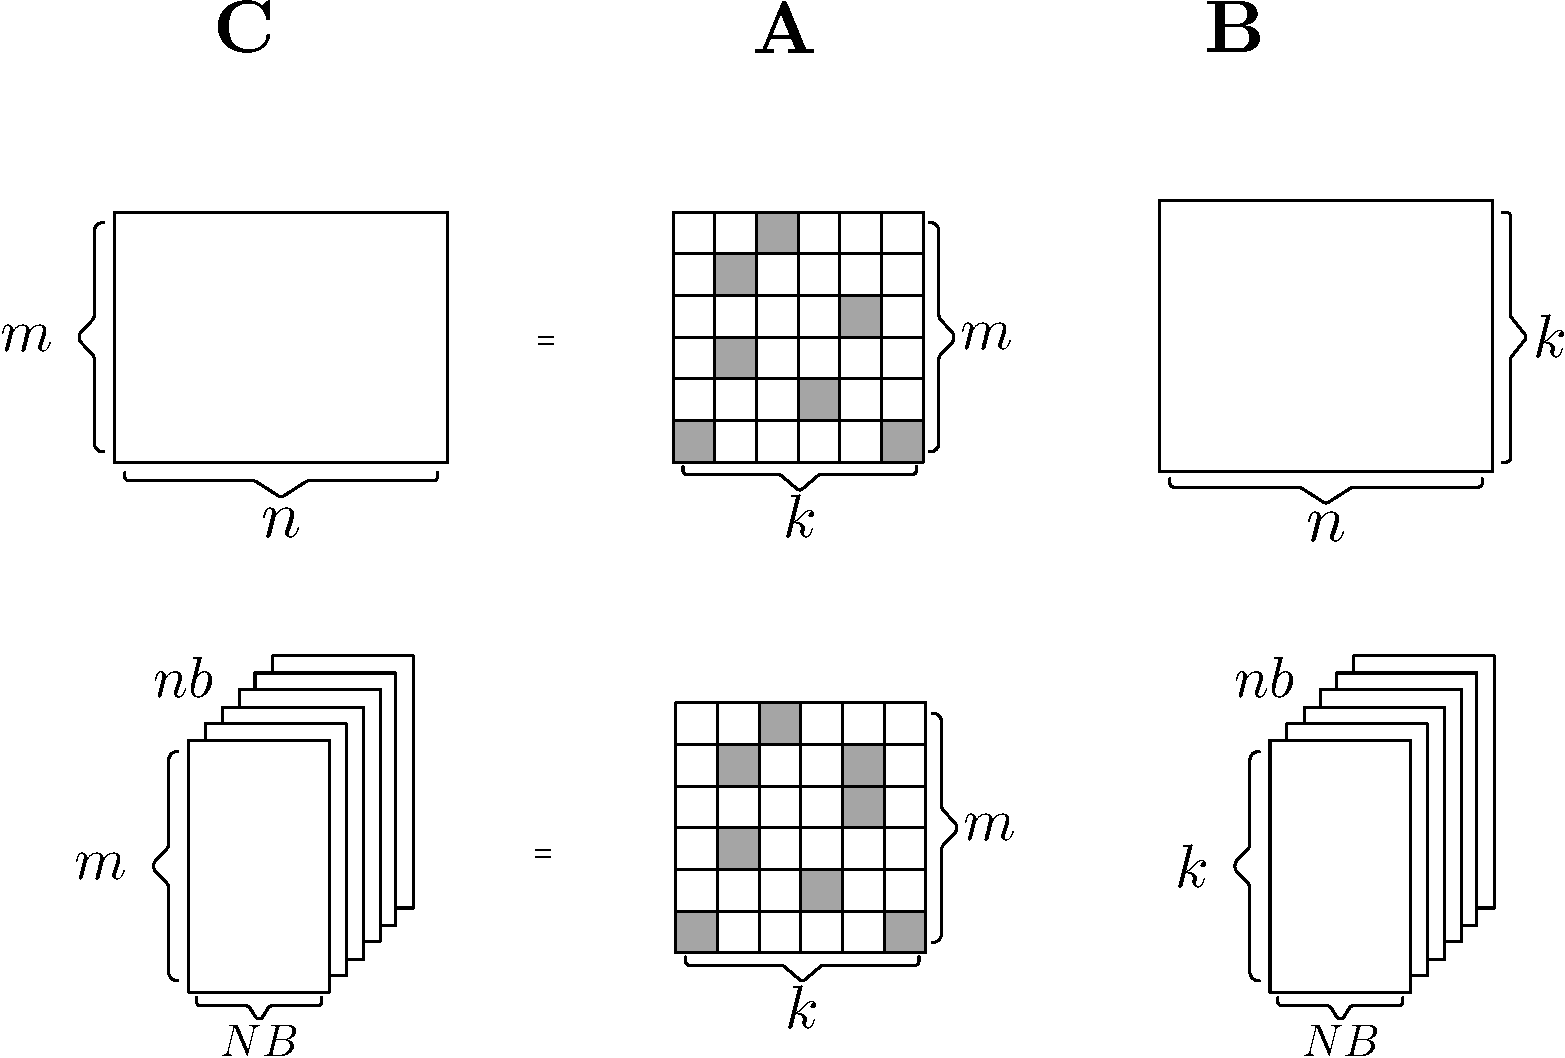
\includegraphics[width=\columnwidth]{imgs/libxsmm_sparse_dense_mult.pdf}
	\caption{LIBXSMM Sparse-Dense Matrix Multiplication (SPMM).}
	\label{fig:libxsmmsparsedense}
\end{figure}

\begin{algorithm}[]
	\KwData{ CSR $A \in \mathbb{R}^{m \times k}$, $B \in \mathbb{R}^{k \times n}$}
	\KwResult{$C \in \mathbb{R}^{m \times n}$  }
	$C[i,k] = 0$\;
	\For{$i = 0$ \KwTo $M-1$}{
		\For{ $j = A.rows[i]$ \KwTo $A.rows[i+1]-1$}{
		  \For{$k = 0$ \KwTo N-1}{
		  	$idx   = A.cols[j]$\;
		  	$C[i,k] \leftarrow C[i,k] +  A.val[j] * I [idx, k]$\;
		  }
		}
	}

	\caption{Sparse-Dense Matrix Multiplication algorithm with CSR format.}
	\label{alg:csr_mult}
\end{algorithm}

%We observe the same problems reported with for dense matrix multiplication in terms of lack of data re-usage. If we observe the most inner cycle computing $C_{i,k}$, we observe that the whole $I$ matrix may be needed to compute the $i$ line of C. As for dense matrix multiplication, a block-wise approach could partially solve this issue. With the lesson learned from the dense case, we can state that we should load data by blocks thus promoting data re-usage. 
%Born in 2015, this library was conceived to cover use cases that other Intel libraries, \textit{e.g.,} MKL and One-DNN, left uncovered. 

\smallskip
\noindent \textbf{Sparse-Dense matrix multiplication with LIBXSMM}. LIBXSMM~\cite{heinecke2016libxsmm} is a high-performance library specifically tailored for Intel architectures, specialized in small dense matrix multiplication, sparse matrix multiplication, and deep learning primitives in general. It is based on ``Just in Time'' (JIT) code specialization, which intends to exploit the runtime information about its operands. The sparse-dense routine was originally developed to solve seismic equations~\cite{breuer2019petaflop}.
% such as matrix shapes or non-zero entires location for sparse matrices. The library includes both dense-sparse and sparse-dense matrix multiplication, and the latter was originally developed to solve seismic equations~\cite{breuer2019petaflop}. 

We now detail the sparse-dense matrix multiplication as implemented in the LIBXSMM library, with A in CSR format. 
The dense matrix $B$ is converted into a three dimensional tensor of shape $k \times N_b \times n_b$, as reported in Figure~\ref{fig:libxsmmsparsedense},
so that $N = N_b \times  n_b$. This means to factorize the $N$ dimension in two sub-dimension, in which one ($n_b$) is induced by the underlying hardware. The ideal value of $n_b$ in fact, coincides with the SIMD length of the processor, \textit{i.e.}, the number of different numbers that a SIMD vector can store. 
Using floating-point variables (32 bit) on a machine with AVX2 ISA (256 bit), the SIMD length is 8. This packing allows to  multiply each non-zero element of $A$  with $nb$ values of $B$ at time, using just one vectorized instruction.



The problem of irregular accesses is tackled by hardwiring the loading of the elements of $A$ and $B$, so that only relevant elements are loaded. The data access pattern provides for multiplying each non-zero element of $A$ ($a_{i,j}$) with the $j$-th rows of $B$ ($B_j$) and accumulate the results into the $i$-th row $C$ ($C_i$).
The computation is carried on one row of $A$ at time. Figure~\ref{fig:libxsmmsparsedensemicro} shows the sub-routine performed for each row $i$.  
Let us call the first non-zero element of the current row $x$, in position $(i,j)$; we assume to have at least one non-zero entry, otherwise the row is skipped. $C_i$ is loaded into $N_b$ SIMD registers, each containing $n_b$ values. $x$ is \emph{broadcasted} to a SIMD CPU register, \textit{i.e.}, $n_b$ consecutive copies of the $x$ vector are loaded into the register. We refer to this vector as $\overline{x}$. 
$B_j$ is loaded as well and $C_i$ is updated as $C_i \leftarrow C_i + \overline{x} B_j$; the update involves $N_b$ Fused Multiply Add (FMA) instructions $C_{i,k} \leftarrow C_{i,k} + \overline{x} B_{j,k}$. Then, the routine moves to the next non-zero elements in the $i$-th row of $A$. Once all the non-zero elements have been multiplied, $C_i$ is stored in memory and the algorithm moves on to the next row of $A$.  


\begin{figure}[t]
\centering
	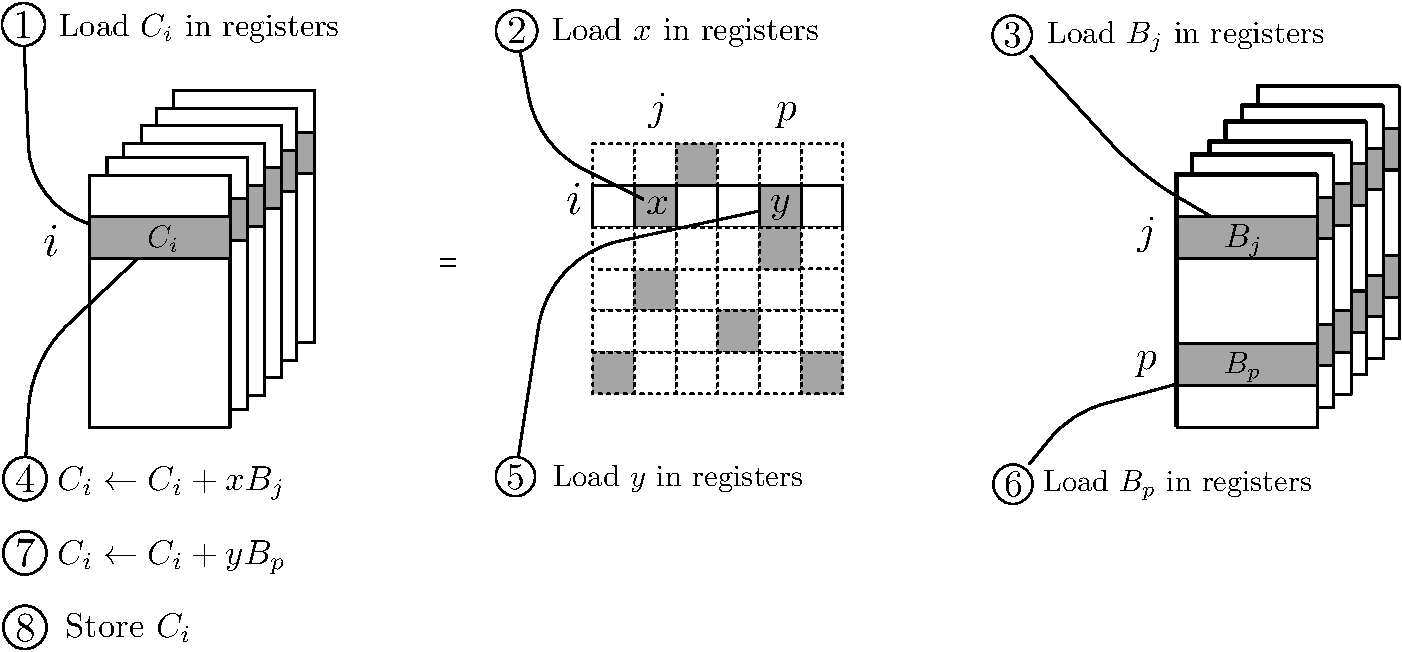
\includegraphics[width=\columnwidth]{imgs/libxsmm_sparse_dense_mult_micro.pdf}
	\caption{Micro Kernel of LIBXSMM Sparse-Dense Matrix Multiplication (SPMM).}
	\label{fig:libxsmmsparsedensemicro}
\end{figure}

LIBXSMM is equipped with a mechanism that interrupts the code generation if the number of instructions is too elevated. This can happen if the number of non-zero elements in $A$ or the $N$ dimension are too large. Since the $N$ dimension corresponds to the batch size in the neural forward, we are free to  reduce it to overcome this limit. When necessary, we also split the $m \times k $ $A$ matrix along the $M$ dimension to generate a set of sub-matrices $A_S = \{A_1, \dots, A_s \ | \  A_i \text{ of size }  M/s \times k  \}$. Each $A_i$ will have fewer non-zero entries, preventing code generation failure. 
 %A==\left(\frac{\frac{\check{A}_{1}}{A_{1}}}{\frac{\vdots}{\check{X}_{M-1}}}\right)
The $C$ matrix is trivially obtained by multiplying each $A_i \in A_S$ with $B$ separately and by stacking the results along the $M$ (vertical) axis:
\[ C = 
  \begin{bmatrix}
    \begin{array}{c}
  A_1 B  \\
  \hline
  A_2 B\\
  \hline 
  \vdots\\
  \hline
  A_s B\\	   
    \end{array}
  \end{bmatrix}
	\]

\smallskip
\noindent \textbf{LIBXSMM vs MKL}. As aforementioned, MKL is known to provide the fastest routine for sparse-dense matrix multiplication. We now show that LIBXSMM outperforms MKL on small, very sparse, and asymmetric matrices, which is the typology of matrices we employ in our MLPs for document scoring. In Table~\ref{table:lib_vs_mkl_msn}, we report the execution time of $C = AB$, with $A$ sparse in the CSR format and B dense, both for MKL and LIBXSMM; on the $x$-axis is reported the shape  ($m \times k $) $A$ and its sparsity. $B$ has shape $k \times n$, where $n$ is the batch size, set to $64$. The matrices correspond to the first layer of real models trained on the \msn dataset~\cite{DBLP:journals/corr/QinL13}, which provides $136$ handcrafted features. The Table shows that LIBXSMM is always faster than MKL on these shapes, with a speedup factor often larger than $2$x. This consideration, together with the availability of the code, has led us to pick the LIBXSMM library as the reference implementation. 

\begin{table}[htb]
	\centering
	\begin{tabular}{llrr}
		\toprule
		\multirow{2}{*}{Shape} &   	\multirow{2}{*}{Sparsity}&  \multicolumn{2}{c}{SDMM Time ($\mu s$)}\\
		\cmidrule{3-4}
		 & & MKL & LIBXSMM \\
		\midrule
		400$\times$136 &  0.996 &         3.1 &          \textbf{1.2} \\
 		300$\times$136 &  0.985 &         2.5 &          \textbf{1.4} \\
 		200$\times$136 &  0.971 &         2.8 &          \textbf{1.6} \\
 		100$\times$136 &  0.989 &         1.0 &          \textbf{0.4} \\
 		50$\times$136  &  0.968 &         0.7 &          \textbf{0.2} \\
 		\bottomrule
	\end{tabular}
	\caption{ Comparison between MKL and LIBXSMM for Sparse Dense Matrix Multiplication (SDMM)	. Shapes and sparsities represent the first layer of FFNs trained on \msn. Batch size is set to $64$.}
	\label{table:lib_vs_mkl_msn}
\end{table}

% \begin{figure}
% \centering
% 	\includegraphics[width=\columnwidth]{imgs/mult_on_\msn.png}
% 	\caption{A comparison between MKL and LIBXSMM. Shapes and sparsities represent the first layer on MLPs trained on \msn. Batch size is set to $64$}
% 	\label{fig:lib_vs_mkl_msn}
% \end{figure}

\subsection{Sparse Time Predictor}
\label{subsec:sptimepred}
In this section, we illustrate the development of a Sparse-Dense matrix multiplication time predictor, specularly for what we have done for the dense case.
As detailed in Section~\ref{subsec:sdmm}, the algorithm provides for iterating over the rows of $A$ with at least one non-zero entry. We start by analyzing the time cost of multiplying the $i$-th row of $A$ with $B$, which is given by the sum of the cost of the following operations. 

\begin{enumerate}
	\item Loading $N_b$ vectorized elements from $C$ (each one of size $n_b$).
	\item Loading each non-zero element in $A_i$. Since the non-zero values of $A$ are stored contiguously in $A.values$, this operation benefits from cache memory.
	\item Loading $N_b$ vectorized elements of $B$ (of size $n_b$) for each non zero element of $A$.
	\item Updating $C_j \leftarrow C_j + x *B_j$, for each $x\neq0$ in $A_i$. Each update consists in $N_b$ FMA instructions. 
	\item Storing $N_b$ vectorized elements of $C$ (each one of size $n_b$).  


\end{enumerate}
Let us define $a_c$ as the set of active columns in $A$, namely the set of columns containing at least one non-zero element, and $a_r$ the set of active rows in $A$. Let us also define $L_c$ as the cost to load and store $N_b$ elements of $C$, $L_a$ the cost of loading one element of $A$ and updating $C_j$ with $N_b$ FMA instructions, and $L_b$ the cost of loading $N_b$ elements of $B$. 
%Observe that $L_b$ depends on the $N_b$ factor: we can remove dependence by dividing by $N_b$, or using configurations in which $N_b$ is fixed. Being $N_b = N/ n_b$, with $N$ the batch size, we will pick the latter option. 
When generalizing the previous costs to the entire matrices, we have to take into account the effects of caching. 
While $A$ and $C$ are loaded just once, $B$ elements can be loaded multiple times; whether they benefit or not from the caching mechanism depends on the access pattern induced by the non-zero entries of $A$.
For example, if $x$ in position $(i,j)$ is a non-zero element, $B_j$ needs to be loaded into the registers from the main memory and the cache will also retain a copy of $B_j$.
Assume that in a successive row of $A$ exists an element $x' \neq 0$ on the same column of $x$, \textit{i.e.} in position $(g, j)$, with arbitrary $g$. When performing $C_g \leftarrow C_g + x' B_j$,  $B_j$ already resides in the cache: since loading elements from the cache is way much faster than loading them from memory, the cost of re-loading $B_j$ can be considered negligible. 
Assuming that once a row of $B$ is loaded into the cache it remains there until the end of the operation, we pay the cost of loading a row $B_j$ just the first time that this row is loaded. At the same time, if there are any inactive rows, they are never used in the multiplication routine. Since the number of active rows in $B$ is equal to the number of active columns of $A$, the cost of loading $B$ can be approximated with $L_b |a_c|$, with $|a_c|$ representing the number of active columns in $A$.

The overall cost of SPMM with the LIBXSMM is given by: 
\begin{equation}
\label{eq:sparsepred}
	T = |a_r| * L_c +  nnz * L_a + |a_c| * L_b
\end{equation}

%is multiplied with the number of active columns. In fact, if we consider $B$ and $C$ to reside in the main memory at the beginning of the operation, once that a line of $B$ has been loaded into the cache it will likely remain into a cache during the rest of the operation. 	

With an accurate estimation of $L_a$, $L_b$, and $L_c$, we can predict the execution time of a sparse-dense matrix multiplication just from the structure of the sparse matrix. Note that this structure is known \textit{a priori}, being the sparse matrices the pruned weights of the neural model. We begin by observing that $L_b$ and $L_c$ both describe memory operations, with the difference that $L_c$ measures both data reading and writing, while $L_b$ refers to data reading. We empirically verify that both the operations have the same time cost, \textit{i.e.}, $L_c = 2 L_b$. 

We now infer the coefficients $L_a, L_b, L_c$, starting from $L_b$. We cannot measure with a timer the cost of the elementary operations we have divided the LIBXSMM SPMM routine in, but we can empirically compute them by difference.

Let us consider two different sparse matrices $A_c$ and $A_{rd}$ with the same shape $m \times k$ and the same number of non-zero entries ($nnz$). $A_c$ has the non-zero values disposed on the same column $j*$, \textit{i.e.}, is a matrix where $a_{i,j} = 0 $ if $j \neq j*$. $A_{rd}$ is a sparse matrix which has single non-zero entry for each row and each column, \textit{i.e.,} $\sum_{i=0}^{i=m-1} a_{i,j} = 1, \forall j=0, \dots, m-1$  and $\sum_{i=0}^{i=k-1} a_{i,j} = 1,  \forall i=0, \dots, k-1$. 
The cost of multiplying $A_c$ and $A_{rd}$
with a dense matrix is given by:
\begin{align}
\nonumber
T (A_c) = m * L_c + nnz *L_a + 1 * L_b \\
\nonumber
T({A_{rd}}) = m * L_c + nnz *L_a + k * L_b
\end{align}
so, 
$$T(A_{rd}) - T({A_c}) =  (k-1) *L_b$$
We can experimentally measure  $T(A_{rd})$ and $T({A_c})$ and use them to compute $L_b$, since $k$ in known. 

To derive $L_a$, we use the same $A_c$ as before and a second matrix $A_{2c}$, having $2*nnz$ non-zero entries, organized along two columns. The cost for multiplying $A_{2c}$ with a dense matrix is given by 
$$T (A_{2c}) = m * L_c + 2*nnz *L_a + 2* L_b$$
Since $L_b$ can be derived using the previous expression, we can subtract $T(A_{2c})$ and $A_c$ and obtain $L_a$ as:
$$L_a = (T(A_{2c} )- T(A_c))/nnz -L_b$$
Our aim is to compute size-agnostic $L_a$, $L_b$ and  $L_c$. We set $M=K$ and vary them in $\{200, 300, 400, 500 \}$ and we experiment $N \in \{16, 32, 64\}$. $L_b$ and $L_c$ depends on $N$ (and so do $L_c$, which is computed doubling $L_b$), so we normalize diving by $N$. We observe that when $N \geq 128$, the value obtained for $L_a$ and $L_b$ diverge w.r.t. to smaller batch size. In fact,  larger $N$ values ($N \geq 128$) break the hypothesis of $B$ residing inside the cache during the whole multiplication, which is a fundamental assumption of our time predictor.  The definitive time predictor parameters are computed as an average of their value obtained with different shape configurations.
We demonstrate the validity of our sparse predictor in Table~\ref{table:est_vs_real_exec_t_sparse}, where we report the predicted and the real execution time needed to multiply the weights of the first layer of several neural models with a random input. We restrain our experiments to the sparsity range obtained with pruning on our neural architectures. As we will detail later, at these sparsity levels the time required for SDMM  is negligible w.r.t. to its dense counterpart. We also evidence that our time predictor is specific to matrix multiplication, hence can be essentially applied to fully-connected layers. Convolution or attention-based architectures have different properties that require a specific investigation. We leave these analyses for future works.

As we can see, the predictor is capable of correctly estimating the execution time of different models at high levels of sparsity, with a small error. Specifically, the predictor can fruitfully distinguish between matrix with the same shape but with different sparsity percentages; two examples are the $200 \times 136$ and the $100 \times 136$ instances in Table~\ref{table:est_vs_real_exec_t_sparse}. First, we observe that with sparsity percentage in the order of $1\%$, SDMM execution times can vary up to $30\%$. Second, the time predictor correctly reflects this peculiarity, thanks to the deep understanding of the routine details that stands behind its development.

% Observe that an exact predictor is beyond the scopes of this paper; its role is just to reduce the neural models search space by dividing them into models which can match an efficiency requirement an models than can not. 

\begin{table}[htb]
	
	%
	
	\adjustbox{max width=\columnwidth}{
	\centering
	\begin{tabular}{lrrrrrrr}
	%\resizebox{\columnwidth}{!}{
		\toprule
		\multirow{3}{*}{Shape} &   	\multirow{3}{*}{Sparsity}& 
		 \multicolumn{6}{c}{SDMM Time ($\mu s$)} \\
		\cmidrule{3-8}
		& & \multicolumn{2}{c} {$N=16$}& \multicolumn{2}{c} {$N=32$} & \multicolumn{2}{c} {$N=64$} \\
		\cmidrule{3-8}
		 & & Real & Pred. & Real & Pred. & Real & Pred.\\		
		 \midrule
		 \multirow{2}{*}{400$\times$136} &  0.995 & 0.2 & 0.2 & 0.4& 0.4&   0.9 &          0.8 
		 \\
		  &  0.986 &  0.4& 0.4& 0.9& 0.8&         1.9 &          1.6 \\
		   \arrayrulecolor{black!30}\midrule

 	300$\times$136 &  0.985 &0.3 &0.3 & 0.7& 0.7&        1.6 &          1.4 \\
 	 	  \arrayrulecolor{black!30}\midrule

 	 	\multirow{2}{*}{200$\times$136} &  0.982 &   0.3& 0.3& 0.5 & 0.5 &        1.0&          1.0 \\
 	  		&  0.971 &       0.4& 0.3& 0.7&0.6 &  1.5 &          1.3 \\
 	  	\arrayrulecolor{black!30}\midrule

 	 	\multirow{2}{*}{100$\times$136} &   0.989 & 0.1 &0.1 & 0.2& 0.2 & 0.5 &          0.4 \\
          &  0.967 & 0.2&0.2 & 0.3& 0.4&      0.7 & 0.7 \\ 
         \arrayrulecolor{black!30}\midrule

 	 	50$\times$136  &  0.987 &0.1 	& 0.1& 0.1 & 0.1 & 	   0.2 & 		  0.2 \\
 	 	\arrayrulecolor{black}
 	 	\bottomrule
	\end{tabular}
	}
	
	\caption{Some examples of our sparse time predictor with different values of $N$.}
	\label{table:est_vs_real_exec_t_sparse}

\end{table}

% \section{Forest Distillation}
% \label{sec:fordist}
% In this section we detail how to train a Feed-Forward Neural Network (FFNN or NN) to score documents in a Information Retrieval (IR) system. The idea was first proposed by Cohen \textit{et al.}~\cite{cohen2018universal}: NNs are known to be universal approximators~\cite{hornik1991approximation}, so they can be trained to mimic the output of an ensemble of regression trees, becoming \textit{de facto} a document scoring engine.

% Formally, 
% let us consider a Learning to Rank dataset $D = (X, Y)$,  $X \in \mathbb{R}^{f}$, where $f$ is the number of extracted feature per document, and $Y \in \mathbb{N}$ is the set of ground truth relevances w.r.t. a query.
% Let  $F: \mathbb{R}^{f} \rightarrow \mathbb{R}$ be the underlying function learned by a Regression Forest during the training, mapping document features to document scores. To generate a neural-based scoring document system, we need the network to approximate this function; this is done 
% by replacing the original $Y$ ground truth with $F(X)$, \textit{i.e.}, substituting the ground truth relevances with the scores of the ensemble of regression trees on the dataset $X$. 
% %to virtually create a new $D_F = (X, F(X))$. 

% Even if this approximation-based approach could seem counterintuitive, it results profitable because of the different \textit{learning styles} between the models.
% There are several approaches in Learning to Rank: \textit{pointwise}, \textit{pairwise} and \textit{listwise}; among them, the \textit{listwise} has demonstrated to consistently outperform the others.  Anyway, neural models show to struggle in directly exploiting it; the divergence of learning styles is mainly expressed by the objective functions, which happen to be non-differentiable in the \textit{listwise} approach, hindering Stochastic Gradient Descent (SGD) to find global minima. 
% %TODO qui dettagli
% Minimizing the mean square error between the network and the tree-based model outputs is a way to overcome the problem: the learning style itself is similar to the \textit{pointwise} approach, but since the $F(\cdot )$ function is learned with a \textit{listwise} one, the final $N(\cdot)$ function expressed by the neural model results more accurate, as empirically proven~\cite{cohen2018universal}. 

% A reason to compose this approximation is to exploit high performing neural forward systems to obtain faster scoring mechanisms. Anyway, when comparing 
% Neural Network forward time with the state of the art 
% %\ross{state-of-the-art? mi pare di si} 
% method for scoring Regression Trees, namely QuickScorer~\cite{lucchese2015quickscorer,dato2016fast,8035185}, Cohen \textit{et al.}~\cite{cohen2018universal} observed that NNs are faster only when their forward pass is performed on GPU. For the reasons explained in Section~\ref{sec:introduction} we leave out the GPU inference from our comparison and  limit it to CPU based-inference systems.

% %wihotut optmizazed usage simd instructions	
% In the original article, the comparison on CPU involved: a) old QuickScorer results (written in C++), without SIMD instructions\footnote{ this is due to code availability issues, since QuickScorer code is not publicly available}, b) neural inference using a Python deep learning framework. 
% Our first contribution is to  obtain a solid and coherent CPU comparison between the two methods by measuring the performance on the same hardware, with inference mechanisms written in same the programming language. % \ross{setting: hardware and programming language ?} 	
% First, we train a Regression Forest on the \msn dataset~\cite{DBLP:journals/corr/QinL13}, using a grid search to explore the parameters space and to achieve the best $F(X)$ as possible. In this phase, we limit the number of leaves to $64$. We use LightGBM~\cite{NIPS2017_6907} to train the models, which performs better than RankLib, the tool used in the original article. For the sake of fairness, we believe that NNs shall compete with the best available Regression Forest, which is capable to learn an optimal $F^*(X)$ function, that could results harder to approximate with respect to a sub-optimal generic $F(X)$.

% %TODO dati sulla grid search?

% Once we got the tree model, we train the Neural Model to mimic $F(X)$. We picked two network architectures, a Large Network with 4 layers of size $\{2000,500,5000,100\}$ and a Small Network with 2 layers of shapes $\{500,100\}$, as in the original work. We adopt the same strategy for randomly generating training data use by Cohen \textit{et al}. 	~\cite{cohen2018universal}. We use Adam~\cite{kingma2014adam} as optimizer, with learning rate $0.001$ and no weight regularization nor dropout~\cite{srivastava2014dropout}; we multiply the learning rate by $\gamma = 0.1$ at epochs $\{50, 80 \}$ and use and early stopping criterion on the validation loss; we used the Pytorch framework to train the neural networks. We activation function, we used RELU6, with $\text{RELU6}(x) = min(max(x,0), 6)$. 

% In the original work, neural models could perform as well as the Regression Forest trained with RankLib in terms of MAP. On the contrary, Table~\ref{table:effect_comp_orwk} shows that Neural Networks struggle in approximating the optimal $F^*(X)$ function, thus providing lower MAP and NDCG@10 values. Metrics are computed with the RankEval python library~\cite{rankeval-sigir17}. This first observation states that the approximation step has a cost in terms of accuracy drop that has to be taken into account in the analysis of the effectiveness efficiency trade-off. 

%  %inducing a remarkable $\Delta$ in terms of both the chosen metrics. \ross{L'uso di $\Delta$ cosi farebeb schifo anche ai greci. Aggiungerei numeri veri e conclusione dell'esperimento.}

% Forward time is computed both through a python implementation, as in the original work, and in our own C++ version of NN forward pass. In particular,  for the python version we use PyTorch CPU forward while they tested it with TensorFlow. Instead, we use the \textit{dnnl\_sgemm} routine from Intel oneDNN framework to implement matrix multiplications in C++, with JIT compilation, always forcing single-thread execution. We used the latest version of QuickScorer~\cite{lucchese2016exploiting} that exploits SIMD instructions.
%  %while for GPU PyTorch was the framework adopted either in this work and in the original one.
% CPU experiments were conducted on a Intel i9-9900K CPU, with AVX2 (latest ISA supported by QuickScorer) instructions, 3.5 GHz, with L1-cache 256KiB, L2-cache 2 MiB, L3-cache 16MiB.  Neural Network scoring time is computed with batch size = 1000.

% Despite the large gap in terms of NDCG@10, the Regression Forest scored with QuickScorer is faster of the Large Network, as illustrated by Table~\ref{table:speed_comp_orwk}. 
% Anyway, we believe that a fair comparison shall involve two models at the same effectiveness level; as reported by Table~\ref{table:speed_comp_orwk},
% we can obtain the same NDCG@10 of the Large model with $150 $ trees and $64$ leaves per tree, and the NDCG@10 of the Small model with $200$ trees with $32$ leaves per tree.  Table~\ref{table:speed_comp_orwk} also shows that Quickscorer scores a document $16x$ faster than the Large Network and $2.75x$ times faster than the Small one.
% Hence, tree-based solutions are to prefer to neural networks. This section seems to leave no room for neural models in the document scoring  task; in the following section, we will provide a methodology to create feed-forward networks than can compete or even outscore both the effectiveness and the efficiency of the ensemble of Regression Forests.


% \begin{table}
% 	\centering 
% 	\begin{tabular}{lrrrr}
% 		\toprule
% 		Model &     NDCG@10 &     MAP 0 & MAP 1\\
% 		\midrule

% 		RF (878 trees, 64 leaves)&    0.5246& 0.6304  &0.6604  	\\
% 		\midrule
% 		Large Network &   0.5198&0.6279   &0.6579  \\
% 		Small Network & 0.5180& 0.6277 &0.6576  \\
% 		\bottomrule
% 	\end{tabular}
	
% 	\caption{Comparison in terms of NDCG@10 and MAP between a Regression Forest (878 trees, 64 leaves) and Neural Networks on \msn. MAP$x$ means that $x$ is the score assigned to non relevant results. }
% 	\label{table:effect_comp_orwk}
% \end{table}

% \begin{table}
% \centering
% %\adjustbox{max width = \columnwidth}{

% 	\begin{tabular}{lrrr}
% 		\toprule
% 		\multirow{2}{*}{Model} & \multirow{2}{*}{NDCG@10}&    \multicolumn{2}{c}{Scoring Time ($\mu s$/ doc)} \\
% 		\cmidrule{3-4}
% 		& & Python & C++ \\
% 		\midrule
% 		RF (878 trees, 64 leaves)& 0.5246 & / &8.2  	\\
% 		\midrule
% 		RF (150 trees, 64 leaves)& 0.5206& / &1.5 	\\
% 		RF (200 trees, 32 leaves)& 0.5181&  /&0.8 \\
% 		\midrule
% 		Large Net & 0.5198  &35.6 & 24.4 \\
% 		Small Net & 0.5180  & 3.7 & 2.2 \\
% 		\bottomrule
% 	\end{tabular}
% 	%	}
% 	\caption{Comparison in terms of Scoring Time between Regression Forests and Neural Networks on \msn.  }
% 	\label{table:speed_comp_orwk}
% \end{table}


\section{Neural Engineering}
\label{sec:neuraleng}
In Section~\ref{sec:introduction}, we claim that ensembles of regression trees consistently outperform, both in terms of effectiveness and efficiency, NNs trained with the method proposed by Cohen \textit{et al.}~\cite{cohen2018universal}, when documents are scored on CPU. In this section, we break down a methodology used to create efficient neural models for ranking that can compete with ensembles of tree-based ones.

\subsection{Approximation of an Ensembles of Trees}
\label{subsec:approxbetter}
We employ the methodology proposed by Cohen \textit{et al.}~\cite{cohen2018universal} to train neural models that approximate the scores of an ensemble of regression trees. This approach is effective since we use a powerful model, \textit{i.e.}, an ensemble of regression trees, and a profitable learning strategy, \textit{i.e.}, a \textit{listwise} approach, to extrinsic the structure of the actual underlying probability distribution. This facilitates the learning process of a simpler model, \textit{i.e.}, a shallow neural network. The idea is inherited from a deep learning compression technique named \textit{Knowledge Distillation}~\cite{bucilua2006model, ba2014deep,DBLP:journals/corr/HintonVD15} in which a small, production-oriented, network (\textit{student}) is trained to mimic the output of a large and effective network (\textit{teacher}).

To fully leverage the benefits of this technique, we train an ensemble of regression trees with the best performance on a validation set without taking into account its efficiency. Then, we use its scores as ground truth in a distillation process that trains our neural models. In Table~\ref{table:imprteacher}, we report the validity of this approach using the \msn dataset~\cite{DBLP:journals/corr/QinL13}, a widely adopted LtR dataset composed of more than 30,000 queries, with about 120 documents per query, where 
each document is a vector of 136 features\footnote{The list of features is available at https://www.microsoft.com/en-us/research/project/mslr/}. We adopt the NDCG@10 as quality metric. First, we observe the difference in terms of ranking precision between: 1) a model trained with a fixed number of leaves, \textit{i.e.}, $64$, 2) the best model we could obtain on the \msn dataset. The latter one, which results to have $256$ leaves per tree, consistently outperforms the $64$-leaves model.
%Then, we report the results when using these two tree-based models as teachers for two different neural networks. 
Increasing the number of leaves in tree-based models allows for a remarkable gain in terms of NDCG@10. Indeed, when scoring a tree-based model with QuickScorer, the execution time scales at least linearly with the number of trees and leaves~\cite{lucchese2015quickscorer,dato2016fast}. Hence, a $256$-leaves model is more than $4$x slower than a $64$-leaves one with the same number of trees. 
In fact, given that the scoring time per document of $64$-leaves models is 8.2 $\mu s$, a $256$-leaves one takes at least $33 \mu s$ to be traversed with QuickScorer.
This means that, when pursuing a trade-off between effectiveness and efficiency, the best solution is the ensemble of $878$ trees with $64$ leaves, due to the linear dependency of the scoring time with respect to the number of leaves. 
%\fnote{da dove vedo la giustificazione sperimentale di questa ultima affermazione sopra? FM \cosimo{Non c'e', non possiamo fare esperimenti con 256 foglie perche' QuickScorer non le supporta. Pero' la citazione rimanda al paper di QuickScorer dove c'e' scritto che il tempo di scoring scala linearmente. Cosimo}. chiaro. metterei i conti della serva per convincere il revisore a spanne che quel 4x, usando lo scoring con 256 non scala una sega. altrimetni si chiede perche' ``unbearable long scoring times''. no?}

Furthermore, we report the results when using two tree-based models as teachers for two different neural networks. 
Our experiments clearly show the positive effects of approximating a more effective \textit{teacher} (Table~\ref{table:imprteacher}). In fact, thanks to the teacher upgrade, the  $1000\times500\times500\times100$ can provide the same ranking precision as the $64$-leaves tree-based model. Observe that the \textit{student} is teacher-agnostic: the architecture of the network is independent w.r.t. the tree-based model which is approximating, and so is the time to perform the forward pass. In conclusion, distilling from a more effective teacher bridges the gap between neural models and ensemble of regression trees in terms of effectiveness. Nevertheless, a margin still exists between the two families of models in terms of efficiency. In the following sections, we will show how to tackle this aspect. 

%we evidence the advantages of  approximating a better \emph{teacher} model, and we incorporate this strategy in our general train and design methodology. Anyway, 
%approximating a better model is an uniquely profitable strategy which allows to improve the effectiveness of the neural models, with no drop in terms of efficiency. 

\begin{table}
% \centering
% \begin{tabular}{lrrr}
% 		\toprule
% 		Model &     NDCG@10 &     MAP 0 & MAP 1 \\
% 		\midrule
% 		878 trees, 64 leaves &    0.5246& 0.6304  &0.6604 	\\
% 		600 trees, 256 leaves &   0.5291&0.6321   &0.6621  \\
% 		\bottomrule
% 	\end{tabular}
% 	\caption{Comparison between Regression Forests with different number of trees and leaves on the \msn dataset}
% 	\label{table:64vs256leaves}
%\vspace{0.6cm}
\centering
%\adjustbox{max width = \columnwidth}{
	\begin{tabular}{llr}
		\toprule
		Model  & Teacher & NDCG@10 \\
		\midrule	
		878 trees, 64 leaves &  / &  0.5246  \\
		600 trees, 256 leaves &  / &  $\uparrow$ \textbf{0.5291}     \\
		\midrule
		\multirow{2}{*}{500$\times$100} & 878 trees, 64 leaves & 0.5180 \\
		& 600 trees, 256 leaves &$\uparrow$ \textbf{0.5198} \\  
		\midrule
		\multirow{2}{*}{100$\times$500$\times$500$\times$100} & 878 trees, 64 leaves & 0.5208 \\
		& 600 trees, 256 leaves &$\uparrow$ \textbf{0.5243}  \\
		\bottomrule
	\end{tabular}
	%	}
	\caption{Comparison in terms of NDCG@10 among Neural Networks on \msn, when trained to approximate different teachers.  $\uparrow$ indicates statistically significant improvement (Fisher's randomization test,  $p < 0.05$).  }
	\label{table:imprteacher}
\end{table}


\subsection{Design of a Neural Model}
\label{subsec::neuraldesign}
In this section, we present our novel methodology to design efficient neural models for ranking. We leverage the insights gained in studying dense and sparse matrix multiplication to show how to make correct architectural choices, thus training a very limited set of candidate models. We provide an empirical evaluation to show the correctness of our assumptions. 
Experiments are conducted on the  \msn dataset~\cite{DBLP:journals/corr/QinL13}, as in Section~\ref{subsec:approxbetter}. We first show how to develop dense models matching some given time requirements. Then, we employ pruning techniques to sparsify these models and outperform ensembles of regression trees.

\smallskip
\noindent \textbf{Architecture design}.
Our approach begins by choosing the dense architectures matching some given time constraints. For the sake of simplicity, we will assume to have two tree-based models to compete with, a $300$-trees ensemble and a $500$-trees ensemble, each one with $64$ leaves per tree. Their NDCG@10  and their scoring time ($\mu s$) are reported in Table~\ref{table:widevsdense}. By using the time predictor developed in Section~\ref{subsec:densetimepred}, the identification of the architectures matching the time requirements is now an easier task.
We build a heatmap as in Figure~\ref{fig:heatmap} and then use it to predict the execution time of the architecture, without the need of testing its performance on real hardware. This allows to discard models that do not match the desired latency constraints. As reported in Table~\ref{table:widevsdense}, there can be several models fitting the time budget. In our case, we propose $2,3,4$ layers NNs. We train the chosen models and compare their NDCG@10. \textit{Deep} networks (more layers) afford better performance w.r.t. \textit{wide} ones (more neurons per layer), coherently with the evolution of neural models witnessed in the last decade. The reason is that deep networks are generally capable of extracting higher levels features thus creating more complex representation of the input. The higher representations are built on simpler ones, generating a nested hierarchy of concepts which allows to improve the understanding and the learning from the data~\cite{Goodfellow-et-al-2016}. We empirically verify that $5$-layers models matching the time constraints do not offer advantages with respect to $4$-layers ones, showing that $4$-layer networks are expressive enough for the ranking task. Dense networks offer performance close to the tree-based model but do not really guarantee advantages neither in terms of effectiveness or efficiency, as shown in Table~\ref{table:widevsdense}.

\begin{table}
\centering
%\adjustbox{max width = \columnwidth}{
	\begin{tabular}{lrr}
		\toprule
		%\multirow{2}{*}{Model}  &  \multicolumn{1}{p{3cm}}{\centering Predicted Execution \\ Time ($\mu s$/doc) }  & \multirow{2}{*}{NDCG@10} \\

		Model & Scoring Time ($\mu s$/doc) & NDCG@10 \\
		\midrule

		QuickScorer 300, 64 & 3.0  & 0.5230	\\
		\cdashlinelr{1-3}
		500$\times$100 & 2.2 & 0.5196 \\%& 2.2 \\
		300$\times$200$\times$100 & 2.4 &  0.5209 \\
		300$\times$150$\times$150$\times$30 & 2.2 & 0.5207 \\
		\midrule
		QuickScorer 500, 64 & 4.9  & 0.5240	\\
		\cdashlinelr{1-3}
		1000$\times$200 & 5.5 & 0.5150 \\
		600$\times$300$\times$100 & 5.6 & 0.5203\\
		500$\times$250$\times$250$\times$100 & 5.4 & 0.5218\\
		\bottomrule
	\end{tabular}
	%	}
	\caption{Comparison in terms of Scoring Time between QuickScorer and Neural Networks on \msn. The notation ''QuickScorer $x,y$'' indicates that $x$ is the number of trees, and $y$ the number of leaves per tree.   }
	\label{table:widevsdense}
\end{table}


\smallskip
\noindent \textbf{Sensitivity analysis and pruning.}
In our experiments, dense models do not reach the performance of ensembles of regression trees scored with QuickScorer. We now address the problem by leveraging the advantages brought by \emph{model compression}, in particular by \emph{network pruning} \cite{DBLP:journals/corr/HanPTD15,DBLP:journals/corr/GuoYC16}, a technique that deeply sparsifies a neural model without incurring in performance degradation. Let us consider the time budget of $3 \mu s $:
we devise a model which exceeds the time budget but affords an NDCG@10 close the $300$ trees model. By mean of pruning, we can move to the sparse domain and benefit of fast Sparse Dense Matrix Multiplication routines (SDMM). As example model, we pick a 400$\times$200$\times$200$\times$100 network: its performance are reported in Table~\ref{table:sparse_400x200x200x100_partial}.
As detailed in Section \ref{subsec:modelcompr}, \textit{magnitude-based} pruning methods deliver high compression rates without accuracy loss. We adopt this family of pruning techniques to sparsify the parameters of our model. Recall that magnitude pruning technique zero-out a given amount of low absolute value weights. The amount of zeroed-out values determines the aggressiveness of the sparsification: the way this aggressiveness is controlled distinguishes between level pruning and threshold-based pruning.
In the case of level pruning, we can explicitly set the sparsity target, \emph{e.g.}, 70\%.
%
%
In the threshold-based magnitude pruning by Han \textit{et al.}~\cite{DBLP:journals/corr/HanPTD15}, instead, we need to chose a statistical based threshold, as detailed in Section~\ref{sec:related}. The choice is generally based on the \textit{sensitivity} of each layer, namely  the property that describes a layer's resistance to sparsification.
We perform two kind of sensitivity analysis: \textit{static} and \textit{dynamic}. Both procedures prune a growing percentage of weights in each layer, one layer at a time, and evaluate the behavior of the partially-pruned model on the validation set. In the static version, there is no re-training~\cite{DBLP:journals/corr/HanPTD15} of the weights that survived the pruning in the chosen layer and the weights in the other layers, while in the dynamic version re-training is applied.
Static analysis is reported on the left side of Figure~\ref{fig:sensitivity}. The sensitivity of each layer appears to decrease as we go deeper into the network, meaning that the first layers suffer the most from sparsification. Dynamic analysis (right side of Figure~\ref{fig:sensitivity}) shows an inverse trend and highlights a peculiar behavior of the first layer: high levels of sparsity in this layer allow the pruned model to outperform the dense one in terms of NDCG@10.  This is an example of a model compression technique acting as regularizer \cite{DBLP:journals/corr/HanPTD15,DBLP:journals/corr/ZhouYGXC17}.
T%his effect is called regularization, \textit{i.e.}, a growth in terms of generalization capabilities by the model. Pruning techniques can induce this feature since they can be seen as an inference-time version of dropout~\cite{srivastava2014dropout}, \textit{i.e.}, a well-known regularization technique.
This effect is especially evident in the first layer as it presents the weights with the largest absolute values among all the other network layers. Observe that the effect of matrix multiplication is dominated by large absolute value entries, and the larger are the values, the larger is their impact. So a reduced number of high absolute weights can well approximate the overall result of matrix multiplication. From a learning point of view, since the network is working on handcrafted features, the sparsification selects just the essential combinations of input features.

\begin{figure}[t]
\begin{minipage}[b]{0.5\columnwidth}
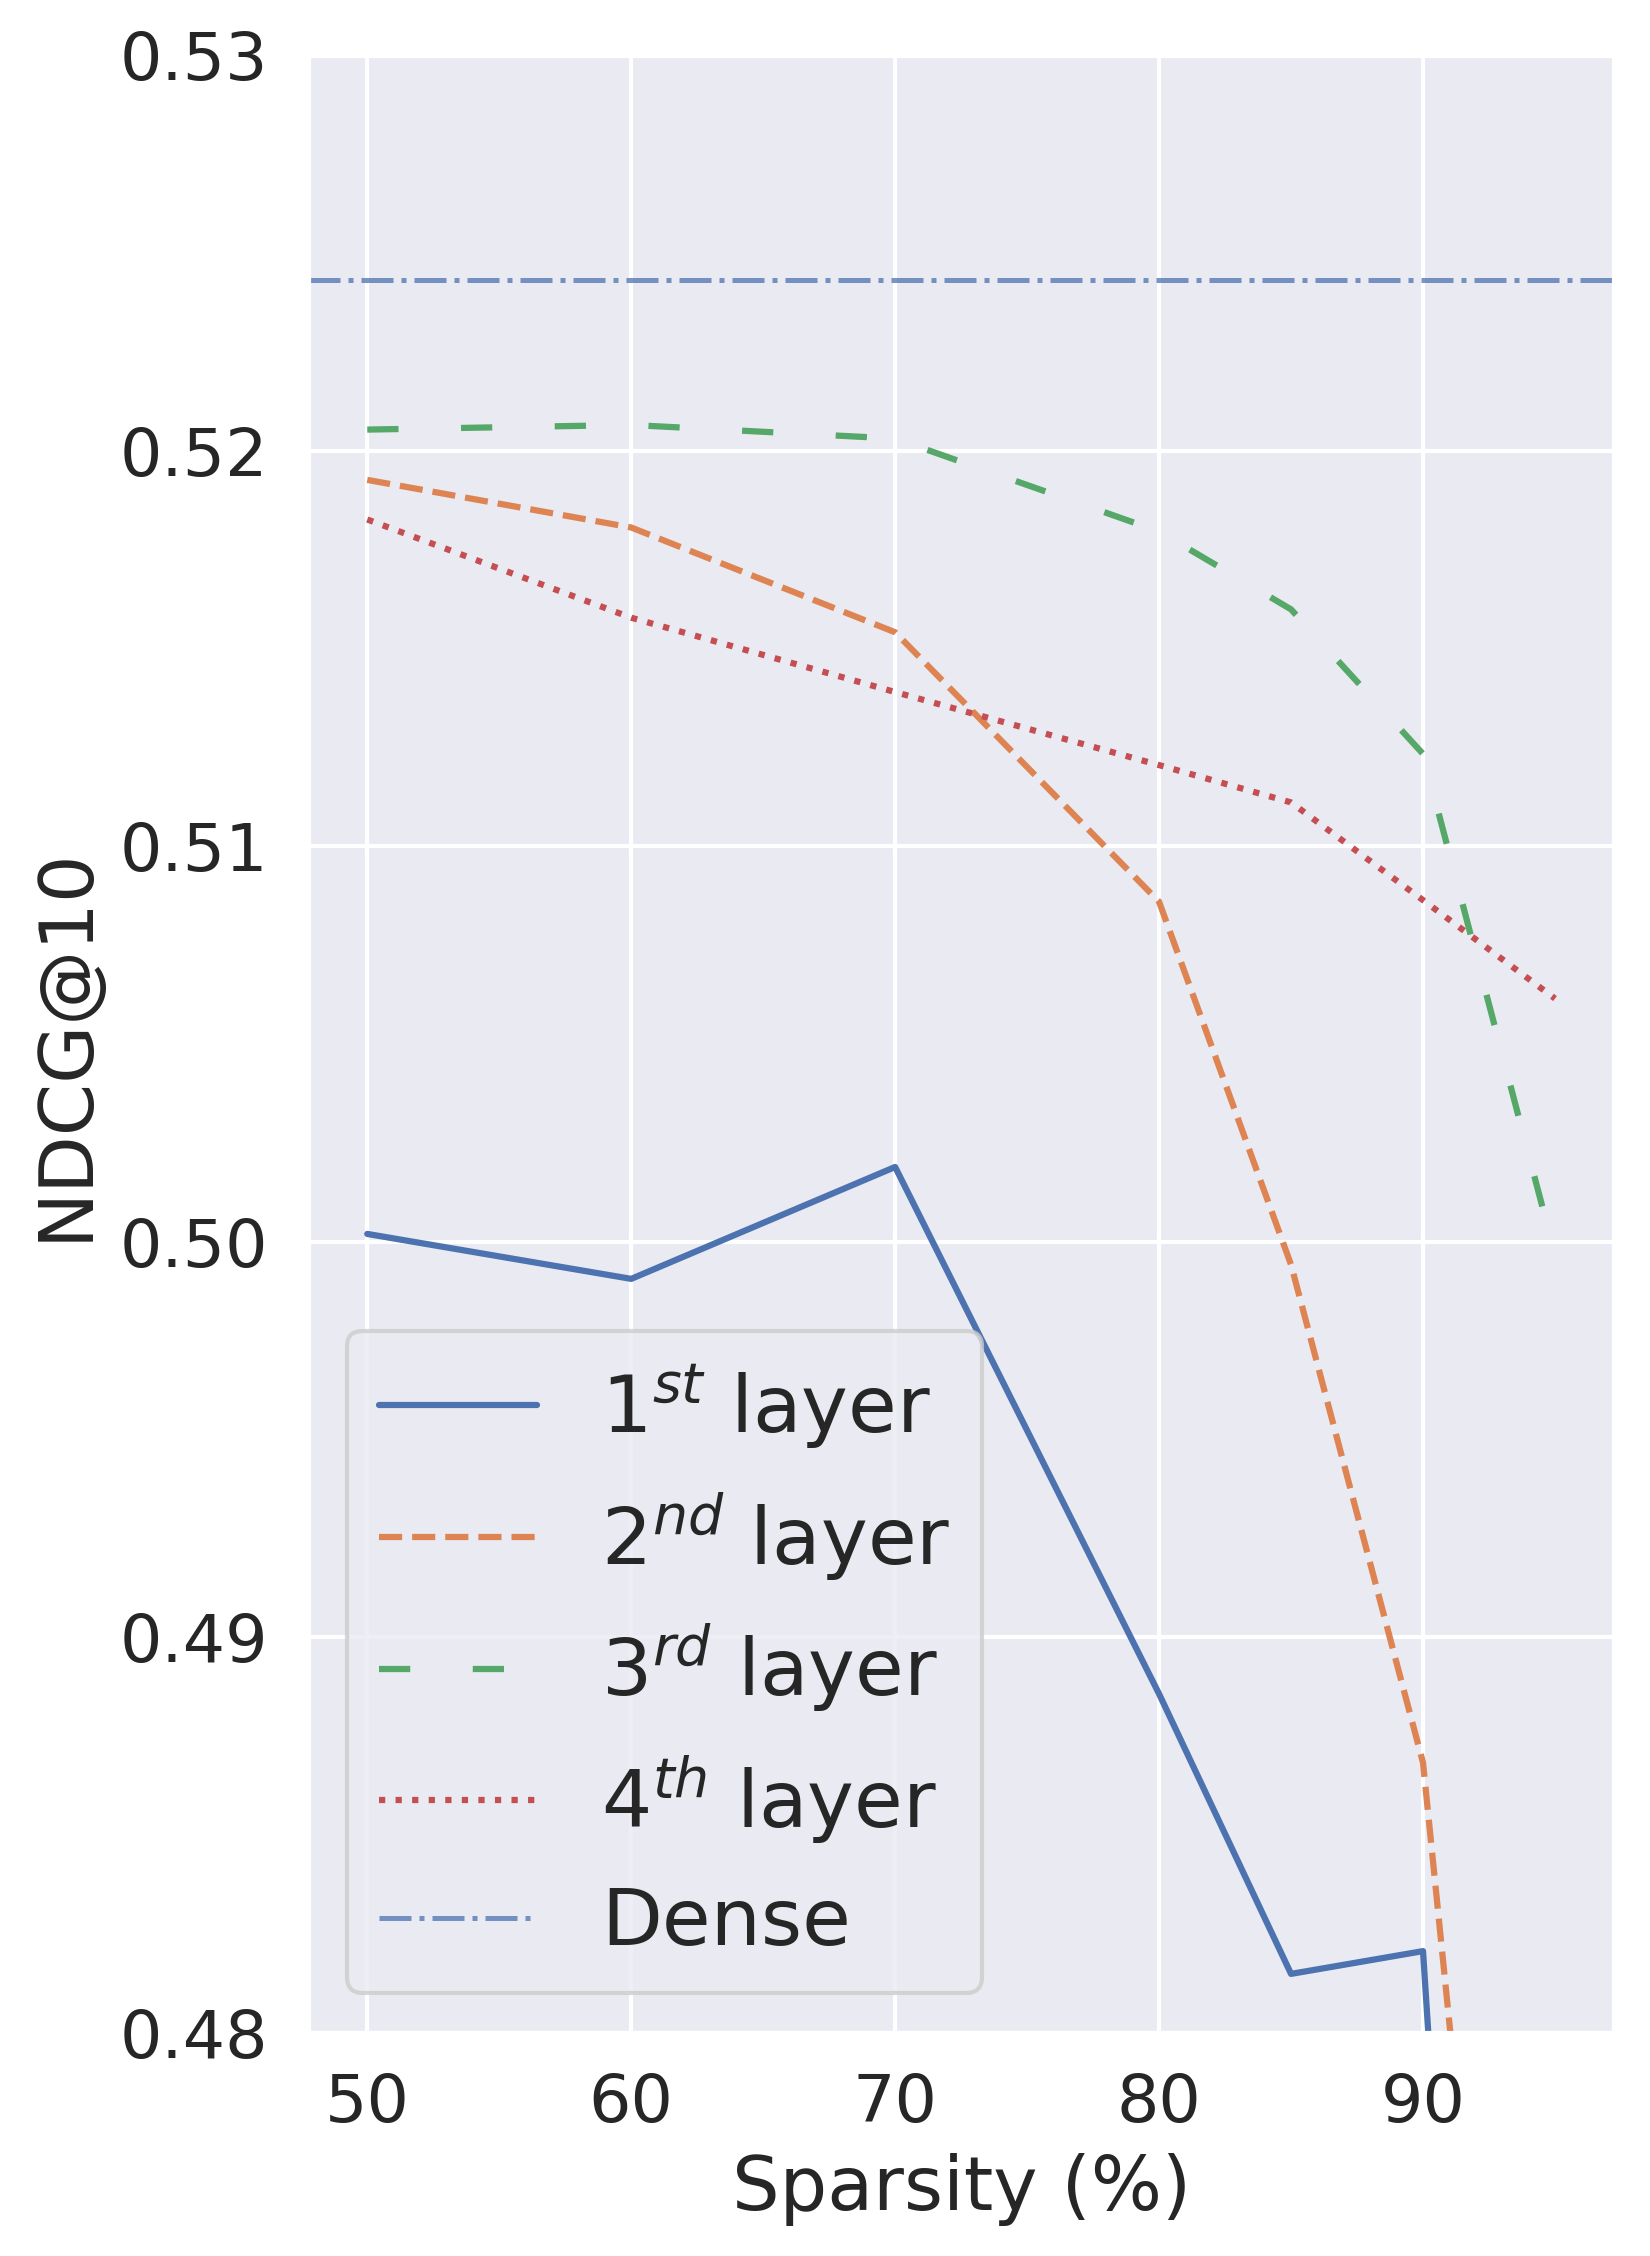
\includegraphics[width=\columnwidth]{imgs/static_sensitivity.png}
\centering 
\caption*{\footnotesize{Static}}
\end{minipage}%
\begin{minipage}[b]{0.5\columnwidth}
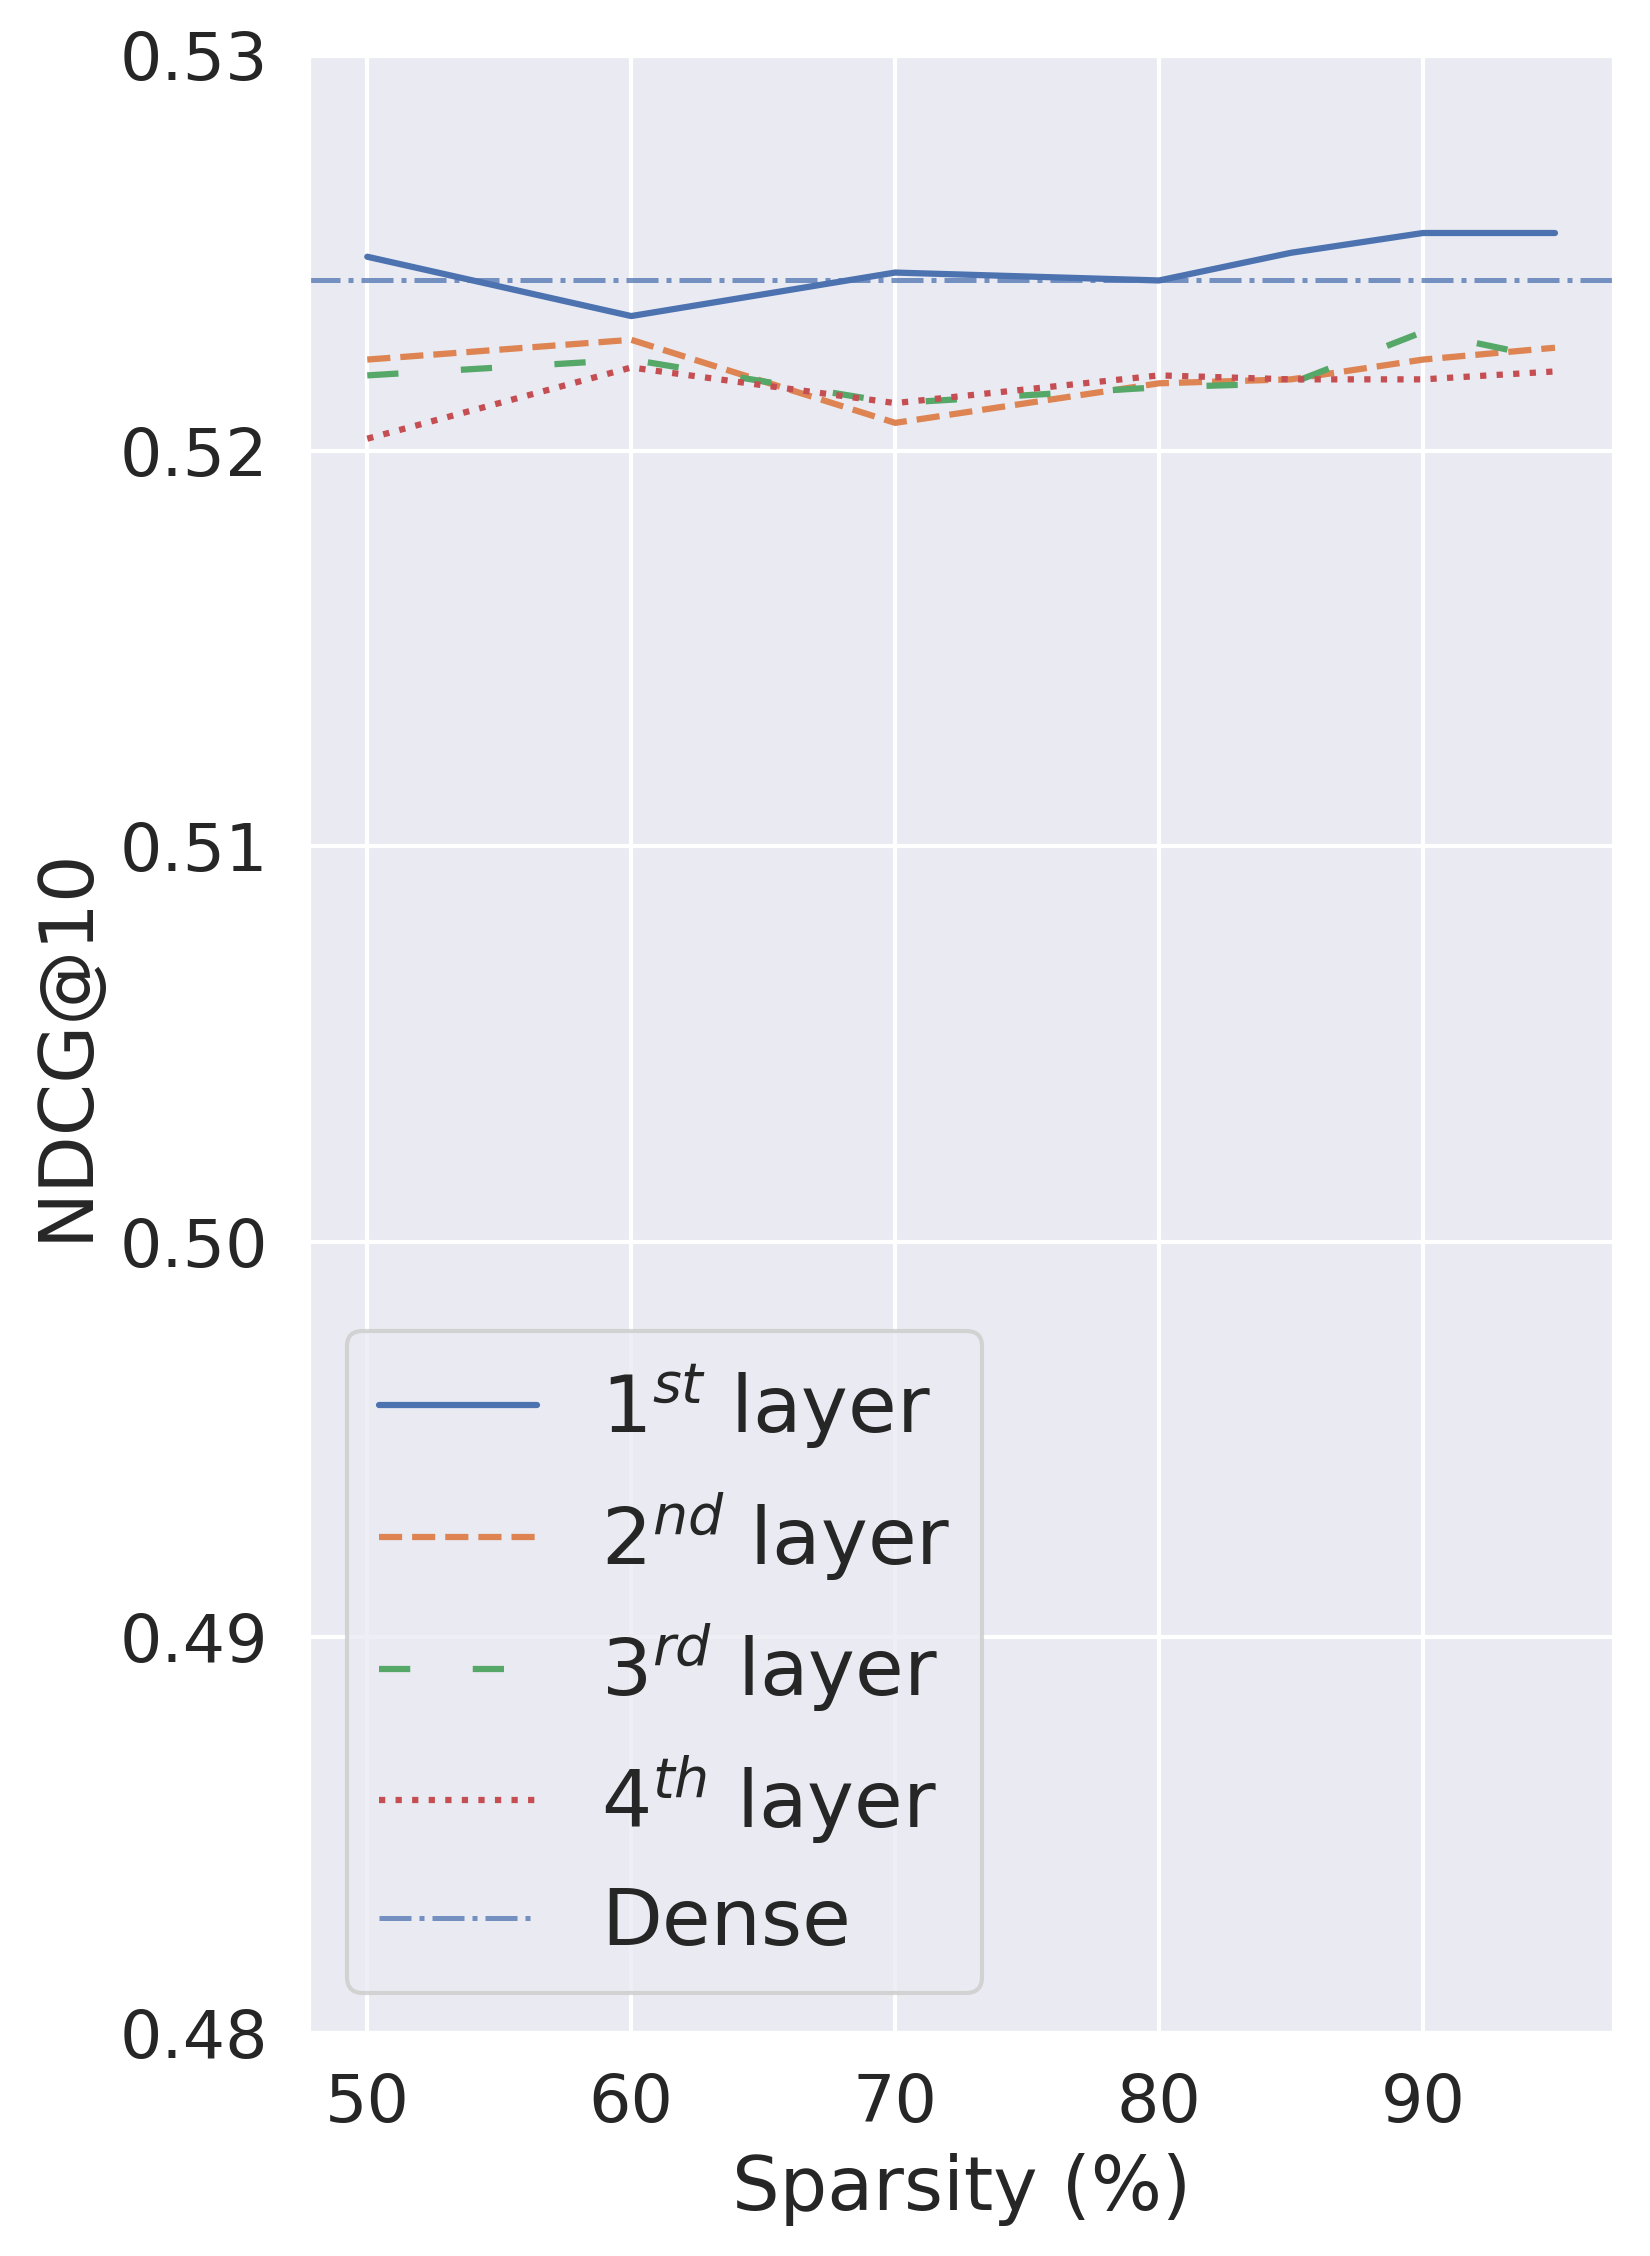
\includegraphics[width=\columnwidth]{imgs/dynamic_sensitivity.png}
\centering 
\caption*{\footnotesize{Dynamic}}
%\subcaption{Another subfigure}
\end{minipage}%
\caption{Static and Dynamic Sensitivity Analysis for a 400$\times$200$\times$200$\times$100 network on the \msn dataset.}
\label{fig:sensitivity}
\end{figure}


\begin{table}[b]
	\centering
	\adjustbox{max width=\columnwidth}{
	\begin{tabular}{lR{0.6cm}R{0.6cm}R{0.6cm}R{0.6cm}R{0.6cm}}
		\toprule
		\multirow{2}{*}{Model} & \multicolumn{5}{c}{\footnotesize{Relative Execution Time per Layer (\%)}} \\
		\cmidrule{2-6}
		 & \nth{1} & \nth{2}& \nth{3} &\nth{4}&\nth{5} \\
		\midrule
		400$\times$200$\times$200$\times$100 & \textbf{35} & 33 & 20 & 10 & 2   \\
		100$\times$50$\times$50$\times$10 & \textbf{60} & 21 & 14 & 3 & 2 \\
		200$\times$100$\times$100$\times$50 & \textbf{45} & 28 & 17 & 8 & 2 \\
		\bottomrule
	\end{tabular}
	 }
	\caption{Breakdown of the relative execution time among different layers for different neural models. }
	\label{table:breakdown}
\end{table}
Pruning techniques were originally developed to reduce the size of pre-trained models~\cite{DBLP:journals/corr/HanPTD15,DBLP:journals/corr/GuoYC16}. %Hence, all network's layers are pruned, even if final sparsities can be low because of high sensitivity of some layers. 
Despite, in our context we aim at speeding up the forward pass without incurring in performance degradation. 
This induces us to consider each layer's relative impact on the inference step before applying a pruning technique. In Table~\ref{table:breakdown}, we report a breakdown of the execution times among different layers in different architectures. Observe that the most time-consuming layer is always the first one, even if the largest matrix is the one storing the second layer weights, as for the 400$\times$200$\times$200$\times$100 network. 
Applying bias and ReLU6, in fact, causes the output matrix of the first layer to be brought into the cache, where it resides there during the computation of the second layer. 
Observe also that it is sufficient to reduce the execution time of one of the first two layers to match the time budget  of $3 \mu s$. By using our sparse time predictor we can infer the required sparsity to obtain a given speedup. In Figure~\ref{fig:sparsespeedup}, we draw the sparsity-speedup curve for some matrices, representing the first layers of different architectures. Even if the dense first layer usually has a major impact on the overall execution time, the quadratic growth of the sparse speedup in the selected range annihilates its contribution after the sparsification. For example, in the 400$\times$200$\times$200$\times$100 architecture, the impact of the first layer in the dense version is about $35\%$, while at $95\%$ of sparsity, the estimated speedup using sparse multiplication is $10$x, meaning that the first layer after pruning becomes the second less time-consuming layer after \textit{fc5}. 



\begin{figure}[t]
\centering
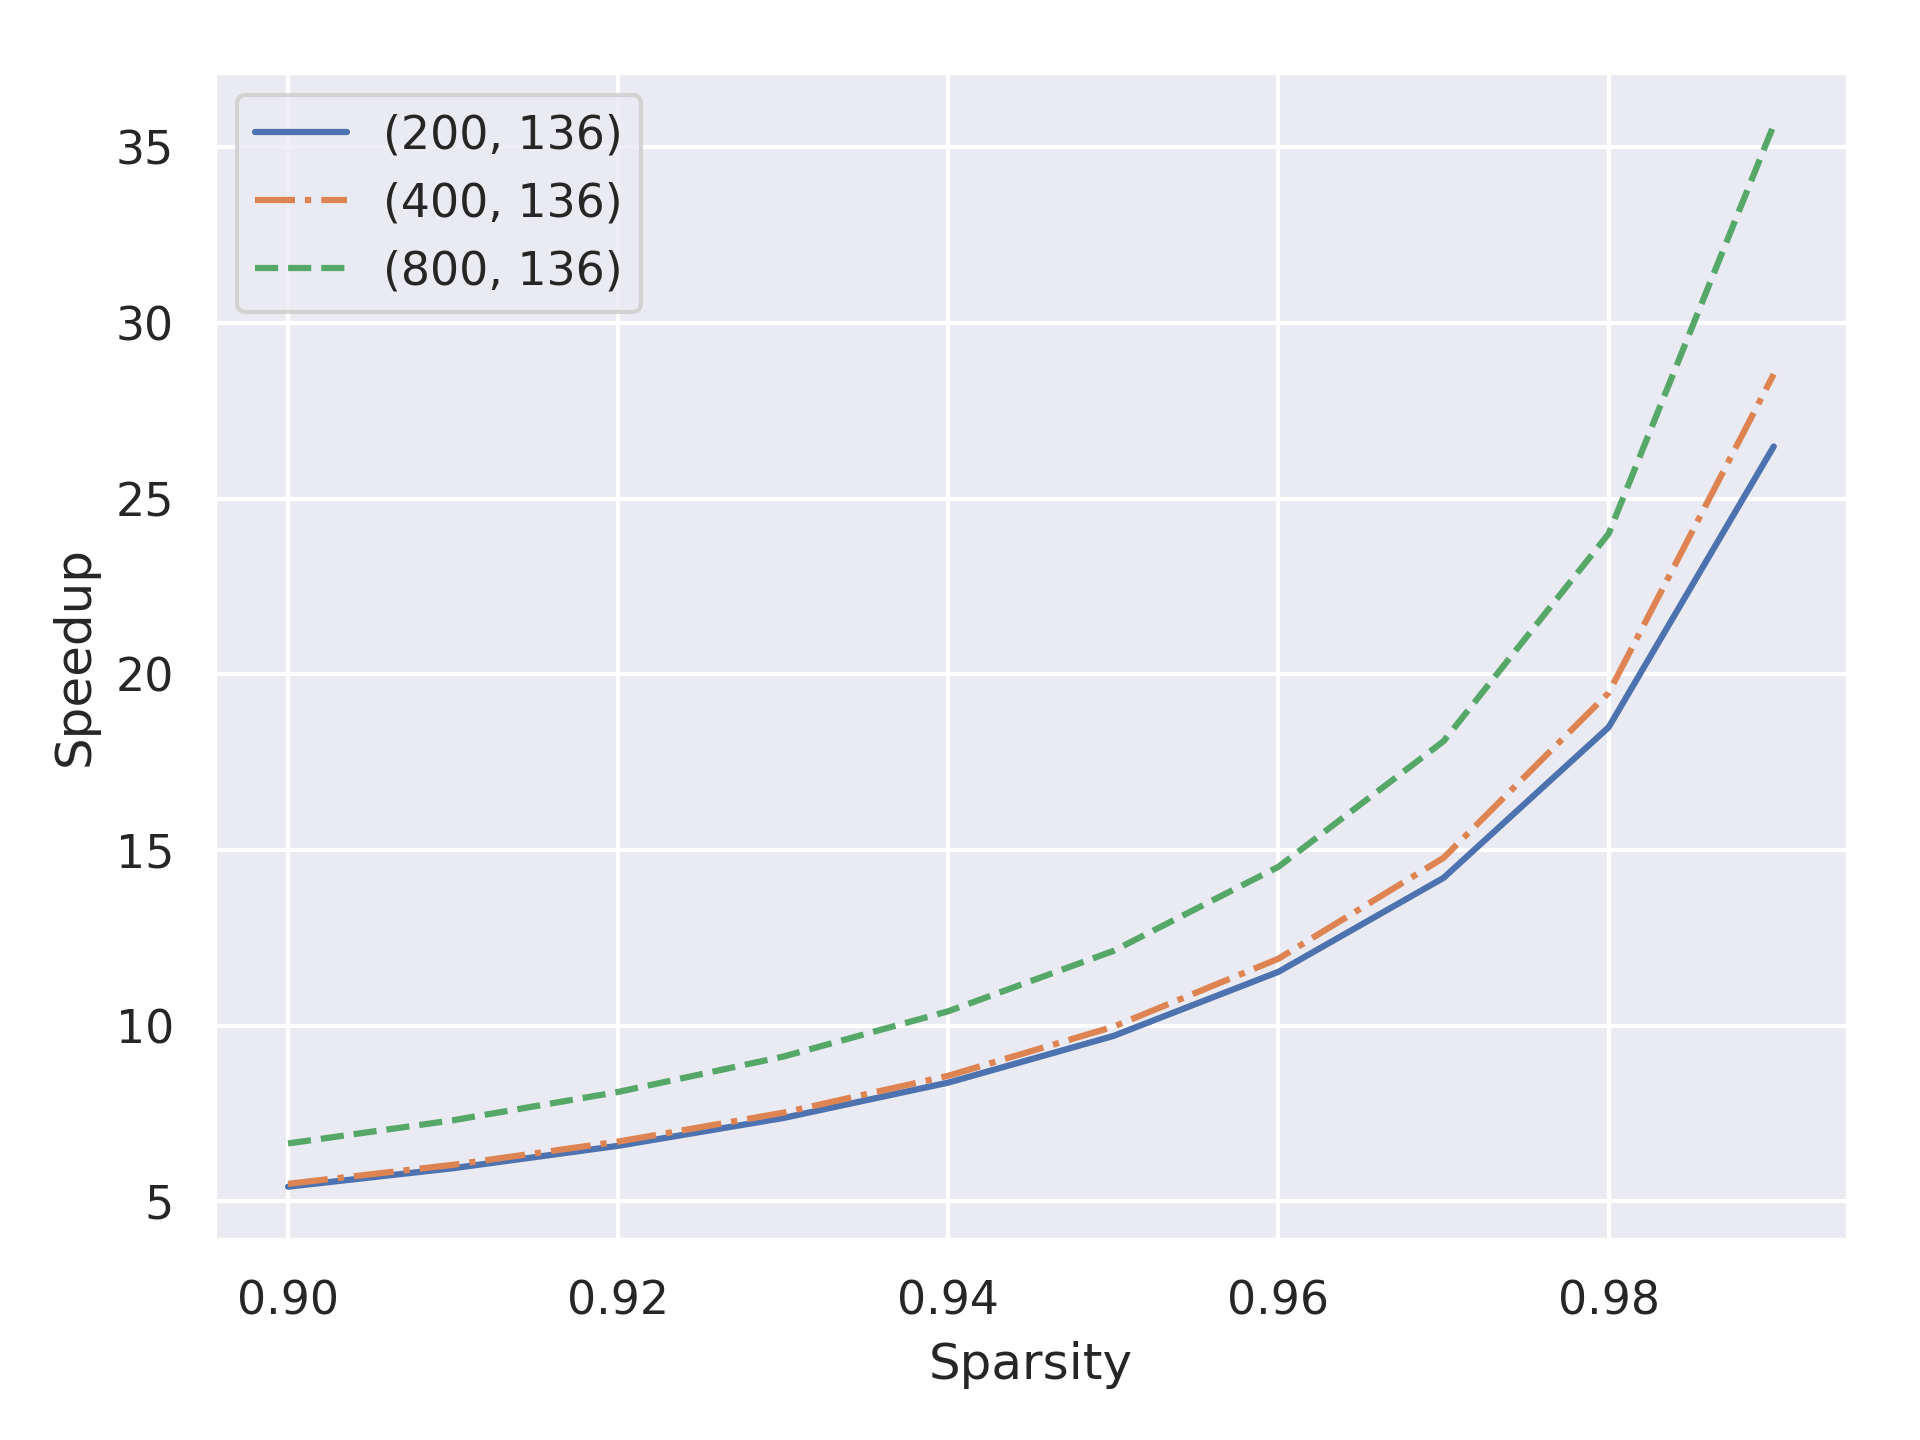
\includegraphics[width=\columnwidth]{imgs/sparse_speedup.png}
\caption{Matrix multiplication speedup at various levels of sparsity estimated with our sparse time predictor. We assume the number of active columns/rows to be equal to the total number of columns/rows (worst-case scenario).\label{fig:sparsespeedup}}
\end{figure}

\smallskip
\noindent \textbf{Outperforming tree-based models}.
By jointly harvesting 1) the prominent impact of the first layer on the total execution time, and 2) the regularization effect of pruning the first layer, we develop our \textit{ early-layers efficiency-oriented pruning}. We apply the threshold-based magnitude pruning using the Distiller framework~\cite{nzmora2019distiller}, a deep learning compression framework developed by Intel. This pruning technique generally offers more flexibility and better performance with respect to level pruning. We prune only the first layer in an aggressive fashion and we fine-tune its surviving entries and all the weights of the other layers.
In our final model, the first layer is $98.7\%$ sparse, meaning that there are about $700$ surviving non-zero weights in the first layer, out of 54400 ($400 \times 136$) in the dense matrix.
We use our sparse time predictor to compute the execution time. The speedup obtained with this sparsity ratio on the multiplication of the first layer is about $25$x. This means that the impact of the first layer, which previously amounted to about the $35\%$, is negligible.
In Table~\ref{table:sparse_400x200x200x100_partial} we report the comparison between tree-based models and neural models. While the dense model did not offer any advantages with respect to the tree-based models, the hybrid model - first layer sparse, other layers dense - is both the fastest and the most accurate model. For example, at the same NDCG@10 value, it is $3.2$x faster than the $878$-trees model. 


\begin{table}[t]
	\centering
	\begin{tabular}{llrr}
		\toprule
		Model & Description & NDCG@10 & Sc. Time ($\mu s$/doc) \\
		\midrule
		\multirow{3}{*}{QuickScorer} & 878 trees & $\uparrow$ \textbf{0.5246} & 8.2 \\
		& 500 trees & 0.5240 & 4.9 \\
		& 300 trees & 0.5230 & 3.0 \\
		\midrule
		\multirow{2}{*}{Neural} & Dense & 0.5222 & 3.8 \\
		& Sparse & $\uparrow$ \textbf{0.5246} & \textbf{2.6} \\ 
 		\bottomrule
	\end{tabular}
	\caption{Dense and sparse neural models (400$\times$200$\times$200$\times$100)  vs QuickScorer in terms of NDCG@10 and Scoring Time (Sc. Time). $\uparrow$ indicates statistically significant improvement w.r.t. models of the same family (Fisher's randomization test,  $p < 0.05$).\label{table:sparse_400x200x200x100_partial}}
\end{table}
